\chapter{Limits of Sequences and Filters}

\section{Closure and Interior}
\subsection{Smallest Open Sets and Largest Closed Sets}



\subsubsection{Smallest Open Subset}

We consider the subset~$B ≔ [0, 1]$ of~$ℝ$.
Let~$U$ be any open subset of~$ℝ$ containing~$B$.
Both end points~$0$ and~$1$ are contained in~$U$, so there exist some radii~$ε, δ > 0$ with~$\ball(0, ε) ⊆ U$ and~$\ball(1, δ) ⊆ U$, and~$ε, δ < 1$.
It follows that the set~$U$ contains the open interval~$(-ε, 1 + δ) = \ball(0, ε) ∪ B ∪ \ball(1, δ)$.
It further follows for the radius~$κ ≔ \min(ε, δ) / 2$ that the open interval~$(-κ, 1 + κ)$ is properly contained in~$U$.

This shows that there exists no open subset of~$ℝ$ that is minimal amongst all open subsets of~$ℝ$ that contain~$B$.



\subsubsection{Largest Closed Subset}

We consider the subset~$B ≔ (0, 1)$ of~$ℝ$.
Let~$C$ be any closed subset of~$ℝ$ contained in~$B$.
The elements~$x ≔ \inf C$ and~$\sup C$ are again contained in~$C$, whence~$0 < x, y < 1$.
It follows that the closed interval~$[x, y]$ is contained in~$B$, with~$C$ contained in~$[x, y]$.
Let~$x'$ and~$y'$ be two real numbers with~$0 < x' < x$ and~$y < y' < 1$.
The closed interval~$[x', y']$ is again contained in~$B$, with~$C$ properly contained in~$[x', y']$.

This shows that there exist no closed subset of~$ℝ$ that is maximal amongst all closed subsets of~$ℝ$ that are contained in~$B$.

\subsection{Closure in Terms of Limit Points}

\begin{proposition}
	\label{closure via intersection with neighbourhoods}
	Let~$X$ be a topological space, let~$B$ be a subset of~$X$ and let~$x$ be a point in~$X$.
	The following conditions on~$x$ and~$B$ are equivalent:
	\begin{equivalenceslist}

		\item
			\label{contained in the closure}
			The point~$x$ in contained in the closure of~$B$.

		\item
			\label{every neighbourhood intersects}
			Every neighbourhood of~$x$ intersects~$B$.

		\item
			\label{every open neighbourhood intersects}
			Every open neighbourhood of~$x$ intersects~$B$.

	\end{equivalenceslist}
\end{proposition}

\begin{proof}
	Conditions~\ref{every neighbourhood intersects} and~\ref{every open neighbourhood intersects} are equivalent because every neighbourhood contains an open neighbourhood.
	We have also the chain of equivalences
	\begin{align*}
		{}&
		x ∉ \closure{B} \\
		\iff{}&
		\text{$x ∉ C$ for some closed subset~$C$ of~$X$ with~$B ⊆ C$} \\
		\iff{}&
		\text{$x ∈ U$ for some open subset~$U$ of~$X$ disjoint to~$B$} \\
		\iff{}&
		\text{some open neighbourhood of~$x$ doesn’t intersect~$B$} \,,
	\end{align*}
	which gives the equivalence of Conditions~\ref{contained in the closure} and~\ref{every open neighbourhood intersects}.
\end{proof}

Let~$X$ be a topological space, let~$B$ be a subset of~$X$, and let~$B'$ be the set of limit points of~$B$.
We have for every point~$x$ of~$X$ the chain of equivalences
\begin{align*}
	{}&
	x ∈ \closure{B}
	\\
	\iff{}&
	\text{every open neighbourhood of~$x$ intersects~$B$}
	\\
	\iff{}&
	\left\{
		\begin{tabular}{@{}l}
			every open neighbourhood of~$x$ intersects~$B ∖ \{ x \}$, \\
			or otherwise~$x ∈ B$
		\end{tabular}
	\right.
	\\
	\iff{}&
	\text{$x ∈ B'$ or~$x ∈ B$} \\
	\iff{}&
	x ∈ B' ∪ B \,.
\end{align*}
This shows the claimed equality~$\closure{B} = B' ∪ B$.


\section{Sequences}
\subsection{Theorem~3.3}

For every open neighbourhood~$U$ of~$x$ there exists some index~$N$ with~$x_n ∈ U$ for every~$n ≥ N$.
This entails that~$U$ and~$\{ x_n \suchthat n ≥ 0 \}$ intersect, whence~$U$ and~$A$ intersect.

This shows that every open neighbourhood of~$x$ intersects the set~$A$, which tells us that~$x$ is contained in the closure of~$A$.

\subsection{Theorem~3.4}

Let~$U$ be an open neighbourhood of~$fx$ in~$Y$.
The preimage~$f^{-1} U$ is an open neighbourhood of~$x$ in~$X$.
Because the sequence~$(x_n)_n$ converges to~$x$, there exists some index~$N$ with~$x_n ∈ f^{-1} U$ for every~$n ≥ N$.
Consequently,~$f x_n ∈ U$ for every~$n ≥ N$.

\subsection{Example~3.4}

\begin{lemma}
	\label{uniquess of sequential limits is inherited by finer topologies}
	Let~$X$ be a set and let~$\top{T}_1$ and~$\top{T}_2$ be two topologies on~$X$.
	Suppose that limits of sequences with respect to~$\top{T}_1$ are unique and that the topology~$\top{T}_2$ is finer than the topology~$\top{T}_1$.
\end{lemma}

\begin{proof}
	Let~$(x_n)_n$ be a sequence in~$X$ with limits~$x$ and~$y$ with respect to~$\top{T}_2$.
	Then~$x$ and~$y$ are also limits of~$(x_n)_n$ with respect to~$\top{T}_1$, since~$\top{T}_1$ is coarser than~$\top{T}_2$.
	Consequently,~$x = y$.
\end{proof}

Let~$X$ be the real line together with the cocountable topology.
Every two proper open subsets of~$X$ intersect (because the union of two countable subsets is again a proper subset of~$X$).
Therefore, no two points of~$X$ can be separated by disjoint open neighbourhoods:
the space~$X$ is very much not a Hausdorff space.

Let~$(x_n)_n$ be a sequence in~$X$ that converges to a point~$x$.
We note that the set~$U ≔ X ∖ \{ x_n \suchthat n ≥ 0 \}$ is open in~$X$, and that the sequence~$(x_n)_n$ never enters the set~$U$.
Therefore,~$x$ cannot lie in~$U$.
More generally, every subsequence~$(x_{k_i})_i$ also converges to~$x$, whence~$x$ cannot be contained in~$X ∖ \{ x_{k_i} \suchthat i ≥ 0 \}$.

The point~$x$ must thus be contained in every subsequence of~$(x_n)_n$.
This is only possible if the sequence~$(x_n)_n$ is eventually constant with value~$x$, i.e., if there exists some index~$N$ with~$x_n = x$ for every~$n ≥ N$.

Consequently, the possible limits of the sequence~$(x_n)_n$ are the same as the limits of the constant sequence~$x, x, \dotsc$
The cocountable topology is finer than the cofinite topology, so it follows from Theorem~3.1 (and the above \cref{uniquess of sequential limits is inherited by finer topologies}) that~$x$ is the unique limit of~$(x_n)_n$.

\subsection{Example~3.5}



\subsubsection{General Observations}

Sawtooth functions correspond to sequences of numbers
\[
	0 < s_1 < r_1 < s_2 < r_2 < \dotsb < s_n < r_n < 1 \,,
\]
where~$n ≥ 1$, the numbers~$r_1, \dotsc, r_n$ are the positions of the vertices, and the numbers~$s_1, \dotsc, s_n$ are the positions of the spikes, see \cref{parametrization of sawtooth functions}.
\begin{figure}
	\centering
	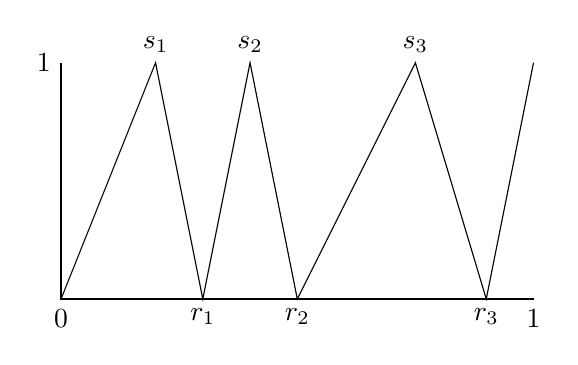
\begin{tikzpicture}[scale = 3, xscale = 2]
		% axis
			\draw[thick] (0, 1) node[left]{$1$} -- (0, 0) node[below]{$0$} -- (1, 0) node[below]{$1$};
		% the line
		\draw (0, 0)
		-- (0.2 , 1) node[above] {$s_1$}
		-- (0.3 , 0) node[below] {$r_1$}
		-- (0.4 , 1) node[above] {$s_2$}
		-- (0.5 , 0) node[below] {$r_2$}
		-- (0.75, 1) node[above] {$s_3$}
		-- (0.9 , 0) node[below] {$r_3$}
		-- (1.0 , 1);
	\end{tikzpicture}
	\caption{Parametrization of sawtooth functions by its vertices and spikes.}
	\label{parametrization of sawtooth functions}
\end{figure}

To describe the closure of~$A$, we will use the following interpolation result.

\begin{proposition}[Interpolation by Sawtooth Functions]
	\label{interpolation via sawtooth functions}
	Let~$n ≥ 1$ be a number of data points, let~$0 < x_1 < \dotsb < x_n < 1$ and let~$y_1, \dotsc, y_n ∈ [0, 1]$.
	There exists a sawtooth function~$f \colon [0, 1] \to [0, 1]$ with~$f x_i = y_i$ for every~$i = 1, \dotsc, n$.
\end{proposition}

\begin{proof}
	Suppose we are given some~$0 < x < 1$ and some~$0 < y < 1$.
	Given~$δ > 0$, there exists a unique line going through the points~$(x - δ, 1)$ and~$(x, y)$.
	This unique line intersects the horizontal line~$ℝ × \{ 1 \}$ at precisely one point, which is of the form~$(x + δ', 0)$ for some~$δ' > 0$, as depicted in \cref{graphical justification for slope formula}.
	We have
	\[
		\frac{y}{δ'} = \frac{1 - y}{δ} \,,
	\]
	and therefore
	\[
		δ' = \frac{y}{1 - y} \, δ \,.
	\]
	\begin{figure}
		\centering
		\begin{tikzpicture}[scale = 3.5, xscale = 1.5];
			% axes
			\draw[thick] (-0.1, 0) node[left] {$0$} -- (1.1, 0);
			\draw[thick] (-0.1, 1) node[left] {$1$} -- (1.1, 1);
			% points
			\draw[fill] (0.2, 1)   ellipse (0.015 and 0.0225) node[above] {$\rightarrow$};
			\draw[fill] (0.5, 0.4) ellipse (0.015 and 0.0225);
			\draw[fill] (0.7, 0)   ellipse (0.015 and 0.0225) node[below] {$\leftarrow$};
			% lines
			\draw (0.5, 0) --node[left] {$y$} (0.5, 0.4) --node[right] {$1 - y$}  (0.5, 1) node[above] {$x$};
			\draw (0.7, 0) -- (0.2, 1);
			% non-visible lines for placement of deltas
			\draw (0.2, 1) --node[above] {$δ$}  (0.5, 1);
			\draw (0.5, 0) --node[below] {$δ'$} (0.7, 0);
		\end{tikzpicture}
		\caption{We have~$y / δ = (1 - y) / δ'$, and as~$δ \to 0$ we also have~$δ' \to 0$.}
		\label{graphical justification for slope formula}
	\end{figure}
	So for~$δ \to 0$ we have also~$δ' \to 0$.

	Let now~$ε > 0$ such that the intervals~$(x_i - ε, x_i + ε)$ are contained in~$[0, 1]$ and pairwise disjoint.
	We define the values~$s_i$ and~$r_i$ as follows:
	\begin{casedistinction}

		\item
			If~$y_i = 0$ then~$s_i ≔ (x_i - ε/2, 1)$ and~$r_i ≔ (x_i, 0) = (x_i, y_i)$.

		\item
			If~$y_i = 1$ then~$s_i ≔ (x_i, 1) = (x_i, y_i)$ and~$r_i ≔ (x_i  + ε/2, 0)$.

		\item
			If~$0 < y_i < 1$, then let~$δ > 0$ be sufficiently small so that both~$δ < ε$ and also~$δ' < ε$ for~$δ' ≔ y / (y - 1) ⋅ δ$.
			We then set~$s_i ≔ (x_i - δ, 1)$ and~$r_i ≔ (x_i + δ', 0)$.

	\end{casedistinction}
	The sawtooth function~$f$ corresponding to the numbers
	\[
		0 < s_1 < r_1 < \dotsb < s_n < r_n < 1
	\]
	satisfies~$f x_i = y_i$ for every~$i = 1, \dotsc, n$.
	See \cref{interpolationg sawtooth function} for an example.
	\begin{figure}
		\[
			\begin{array}{crcr}
				{}
				&
				\centerbox{
				\begin{tikzpicture}[scale = 2.5, xscale = 2]
					% gray areas
					%\draw[fill, gray!30] (0.1, 1) rectangle (0.3, 0);
					%\draw[fill, gray!30] (0.4, 1) rectangle (0.6, 0);
					%\draw[fill, gray!30] (0.7, 1) rectangle (0.9, 0);
					% axes
					\draw[thick] (0, 1) -- (0, 0) -- (1, 0);
					% the points to be interpolated
					\draw[fill] (0.2, 0)   ellipse (0.015 and 0.03);
					\draw[fill] (0.5, 0.5) ellipse (0.015 and 0.03);
					\draw[fill] (0.8, 1)   ellipse (0.015 and 0.03);
					% the intervals with ε = 0.1
					%\draw[(-)] (0.1, -0.2) -- (0.3, -0.2);
					%\draw[(-)] (0.4, -0.2) -- (0.6, -0.2);
					%\draw[(-)] (0.7, -0.2) -- (0.9, -0.2);
				\end{tikzpicture}
				}
				&
				\leadsto
				&
				\centerbox{
				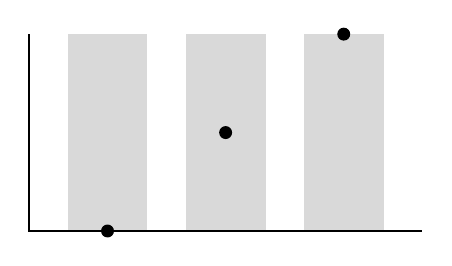
\begin{tikzpicture}[scale = 2.5, xscale = 2]
					% gray areas
					\draw[fill, gray!30] (0.1, 1) rectangle (0.3, 0);
					\draw[fill, gray!30] (0.4, 1) rectangle (0.6, 0);
					\draw[fill, gray!30] (0.7, 1) rectangle (0.9, 0);
					% axes
					\draw[thick] (0, 1) -- (0, 0) -- (1, 0);
					% the points to be interpolated
					\draw[fill] (0.2, 0)   ellipse (0.015 and 0.03);
					\draw[fill] (0.5, 0.5) ellipse (0.015 and 0.03);
					\draw[fill] (0.8, 1)   ellipse (0.015 and 0.03);
					% the intervals with ε = 0.1
					%\draw[(-)] (0.1, -0.2) -- (0.3, -0.2);
					%\draw[(-)] (0.4, -0.2) -- (0.6, -0.2);
					%\draw[(-)] (0.7, -0.2) -- (0.9, -0.2);
				\end{tikzpicture}
				}
				\\[5em]
				\leadsto
				&
				\centerbox{
				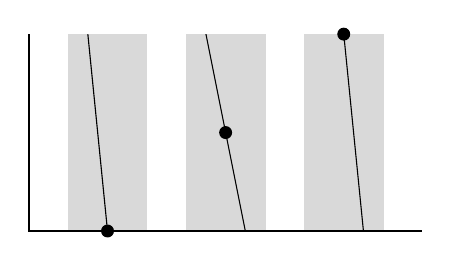
\begin{tikzpicture}[scale = 2.5, xscale = 2]
					% gray areas
					\draw[fill, gray!30] (0.1, 1) rectangle (0.3, 0);
					\draw[fill, gray!30] (0.4, 1) rectangle (0.6, 0);
					\draw[fill, gray!30] (0.7, 1) rectangle (0.9, 0);
					% axes
					\draw[thick] (0, 1) -- (0, 0) -- (1, 0);
					% the points to be interpolated
					\draw[fill] (0.2, 0)   ellipse (0.015 and 0.03);
					\draw[fill] (0.5, 0.5) ellipse (0.015 and 0.03);
					\draw[fill] (0.8, 1)   ellipse (0.015 and 0.03);
					% the intervals with ε = 0.1
					%\draw[(-)] (0.1, -0.2) -- (0.3, -0.2);
					%\draw[(-)] (0.4, -0.2) -- (0.6, -0.2);
					%\draw[(-)] (0.7, -0.2) -- (0.9, -0.2);
					% lines
					\draw (0.15, 1) -- (0.2,  0);
					\draw (0.45, 1) -- (0.55, 0);
					\draw (0.8,  1) -- (0.85, 0);
				\end{tikzpicture}
				}
				&
				\leadsto
				&
				\centerbox{
				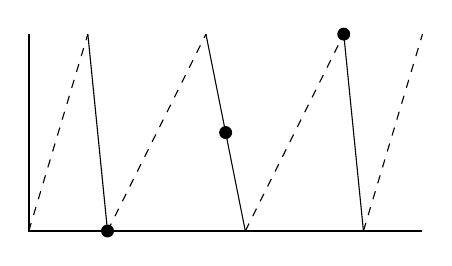
\begin{tikzpicture}[scale = 2.5, xscale = 2]
					% gray areas
					%\draw[fill, gray!30] (0.1, 1) rectangle (0.3, 0);
					%\draw[fill, gray!30] (0.4, 1) rectangle (0.6, 0);
					%\draw[fill, gray!30] (0.7, 1) rectangle (0.9, 0);
					% axes
					\draw[thick] (0, 1) -- (0, 0) -- (1, 0);
					% the points to be interpolated
					\draw[fill] (0.2, 0)   ellipse (0.015 and 0.03);
					\draw[fill] (0.5, 0.5) ellipse (0.015 and 0.03);
					\draw[fill] (0.8, 1)   ellipse (0.015 and 0.03);
					% the intervals with ε = 0.1
					%\draw[(-)] (0.1, -0.2) -- (0.3, -0.2);
					%\draw[(-)] (0.4, -0.2) -- (0.6, -0.2);
					%\draw[(-)] (0.7, -0.2) -- (0.9, -0.2);
					% lines
					\draw (0.15, 1) -- (0.2,  0);
					\draw (0.45, 1) -- (0.55, 0);
					\draw (0.8,  1) -- (0.85, 0);
					\draw[dashed] (0,    0) -- (0.15, 1);
					\draw[dashed] (0.2,  0) -- (0.45, 1);
					\draw[dashed] (0.55, 0) -- (0.8,  1);
					\draw[dashed] (0.85, 0) -- (1,    1);
				\end{tikzpicture}
				}
			\end{array}
		\]
		\caption{A sawtooth function that interpolated between for the three points~$(0.2, 0)$,~$(0.5, 0.5)$ and~$(0.8, 1)$.}
		\label{interpolationg sawtooth function}
	\end{figure}
\end{proof}



\subsubsection{The Closure of~$A$}

Instead of only showing that the zero function lies in the closure in~$A$, we show more generally that~$A$ is dense in~$X$.
To this end, we characterize dense subsets in terms of their intersection with open sets:

\begin{lemma}
	Let~$X$ be a topological space and let~$D$ be a subset of~$X$.
	The set~$D$ is dense in~$X$ if and only if every nonempty open subset of~$X$ intersects~$D$.
\end{lemma}

In other words:
the definition of \enquote{dense} we gave in \cref{definition of dense subsets} is equivalent to the definition given in Section~3.1 the book.

\begin{proof}
	We have the chain of equivalences
	\begin{align*}
		{}&
		\text{$D$ is dense in~$X$} \\
		\iff{}&
		\closure{D} = X \\
		\iff{}&
		\text{the only closed subset of~$X$ that contains~$D$ is~$X$ itself} \\
		\iff{}&
		\text{the only open subset of~$X$ that doesn’t intersect~$D$ is~$∅$} \,,
	\end{align*}
	which proves the assertion.
\end{proof}

Let now~$U$ be any nonempty open subset of~$[0, 1]^{[0, 1]}$.
We need to show that~$A$ intersects~$U$.
For this, we may assume that~$U$ is a basic open set for the product topology, i.e., that there exist distinct points~$x_1, \dotsc, x_n$ in~$[0, 1]$ and open subsets~$U_1, \dotsc, U_n$ of~$[0, 1]$ with
\[
	U
	=
	\{
		f ∈ [0, 1]^{[0, 1]}
		\suchthat
		\text{$f x_i ∈ U_i$ for every~$i$}
	\} \,.
\]
The neighbourhood~$U$ is nonempty, so the sets~$U_i$ must also be nonempty.
For every index~$i$ we choose some point~$y_i$ in~$U_i$.
We know from \cref{interpolation via sawtooth functions} that there exist a sawtooth function~$f$ with~$f x_i = y_i$ for every~$i$, and thus~$f ∈ U$.
This shows that~$U$ intersects~$A$.



\subsubsection{The Zero Function is Not The Limit of a Sequence in~$A$}

\begin{proposition}
	\label{convergece of sequences in products is coordinate-wise}
	Let~$(X_α)_{α ∈ A}$ be a family of topological spaces, let~$(x_n)_n$ be a sequence in~$X ≔ ∏_{α ∈ A} X_α$, and let~$x$ be some point in~$X$.
	Then~$(x_n)_n \to x$ in~$X$ if and only if this holds in each coordinate.
	More explicitly, if~$x_n = (x_n^α)_α$ and~$x = (x^α)_α$, then~$(x_n)_n \to x$ if and only if~$(x_n^α)_α \to x^α$ for every index~$α ∈ A$.
\end{proposition}

\begin{proof}
	For all distinct indices~$α_1, \dotsc, α_r ∈ A$ and all open subsets~$U_i ⊆ X_{α_i}$ we denote the resulting basic open subset of~$X$ by
	\[
		P(U_1, \dotsc, U_r)
		≔
		∏_{α ∈ A}
		\begin{cases*}
			U_i & if~$α = α_i$ for some~$i$, \\
			X_α & otherwise.
		\end{cases*}
	\]
	We have the chain of equivalences
	\begingroup
	\allowdisplaybreaks
	\begin{align*}
		{}&
		(x_n)_n \to x
		\\
		\iff{}&
		\left\{
		\begin{tabular}{l}
			for every open subset~$U$ of~$X$ with~$x ∈ U$, \\
			there exists some~$N$ with~$x_n ∈ U$ for every~$n ≥ N$
		\end{tabular}
		\right.
		\\
		\iff{}&
		\left\{
		\begin{tabular}{l}
			for every basic open subset~$U$ of~$X$ with~$x ∈ U$, \\
			there exists some~$N$ with~$x_n ∈ U$ for every~$n ≥ N$
		\end{tabular}
		\right.
		\\
		\iff{}&
		\left\{
		\begin{tabular}{l}
			for all distinct indices~$α_1, \dotsc, α_r ∈ A$ \\
			and open subsets~$U_i ⊆ X_{α_i}$ with~$x ∈ P(U_1, \dotsc, U_r)$, \\
			there exists some~$N$ with~$x_n ∈ P(U_1, \dotsc, U_r)$ for every~$n ≥ N$
		\end{tabular}
		\right.
		\\
		\iff{}&
		\left\{
		\begin{tabular}{l}
			for all distinct indices~$α_1, \dotsc, α_r ∈ A$ \\
			and open subsets~$U_i ⊆ X_{α_i}$ with~$x^{α_i} ∈ U_i$ for every~$i$, \\
			there exists some~$N$ with~$x_n^{α_i} ∈ U_i$ for all~$i$ and~$n ≥ N$
		\end{tabular}
		\right.
		\\
		\iff{}&
		\left\{
		\begin{tabular}{l}
			for all distinct indices~$α_1, \dotsc, α_r ∈ A$ \\
			and open subsets~$U_i ⊆ X_{α_i}$ with~$x^{α_i} ∈ U_i$ for every~$i$, \\
			there exists some~$N_1, \dotsc, N_r$ with~$x_n^{α_i} ∈ U_i$ for all~$i$ and ~$n ≥ N_i$
		\end{tabular}
		\right.
		\\
		\iff{}&
		\left\{
		\begin{tabular}{l}
			for every index~$α ∈ A$ \\
			and every open subset~$U ⊆ X_α$ with~$x^α ∈ U$, \\
			there exists some~$N$ with~$x_n^α ∈ U$ for every~$n ≥ N$
		\end{tabular}
		\right.
		\\
		\iff{}&
		\text{$(x_n^α)_n \to x^α$ for every~$α ∈ A$} \,.
	\end{align*}
	\endgroup
	This shows the claimed equivalence.
\end{proof}

Suppose there exists a sequence of sawtooth functions~$(f_n)_n$ with~$(f_n)_n \to 0$ with respect to the product topology on~$[0, 1]^{[0, 1]}$.
According to the above \lcnamecref{convergece of sequences in products is coordinate-wise} this is equivalent to~$(f_n)_n \to 0$ pointwise.
However, we will see in the following that this cannot happen, since sawtooth functions are rather rigid:
not too many values of~$f_n$ can tend to~$0$ at the same time.

There exists by assumption for every point~$x$ in~$[0, 1]$ some natural number~$N$ such that~$f_n x ≤ 1/2$ for every~$n ≥ N$.
For every natural number~$N$ let
\[
	B_N
	≔
	\{ x ∈ [0, 1] \suchthat \text{$f_n x ≤ 1/2$ for every~$n ≥ N$} \} \,.
\]
These sets~$B_N$ form an increasing filtration of~$[0, 1]$, i.e., we have
\[
	B_0 ⊆ B_1 ⊆ B_2 ⊆ B_3 ⊆ \dotsb
\]
and~$[0, 1] = ⋃_{N = 0}^∞ B_N$.
We can also describe the sets~$B_N$ in terms of the sets
\[
	B'_n ≔ \{ x ∈ [0, 1] \suchthat f_n x ≤ 1/2 \}
\]
as the intersection~$B_N = ⋂_{n ≥ N} B'_n$.

We note that each set~$B'_n$ is Lebesgue-measurable, since the sawtooth function~$f_n$ is continuous.
Let us calculate the Lebesgue-measure of~$B'_n$:

We observe that for every sawtooth function~$f$ with corresponding points
\[
	0 < s_1 < r_1 < s_2 < r_2 < \dotsb < s_n < r_n < 1 \,,
\]
we have for the set~$B' ≔ \{ x ∈ [0, 1] \suchthat f x ≤ 1/2 \}$ the explicit description
\[
	B'
	=
	\biggl[ 0, \frac{s_1}{2} \biggr]
	∪ \biggl[ \frac{s_1 + r_1}{2}, \frac{r_1 + s_2}{2} \biggr]
	∪ \biggl[ \frac{s_2 + r_2}{2}, \frac{r_2 + s_3}{2} \biggr]
	∪ \dotsb
	∪ \biggl[ \frac{s_n + r_n}{2}, \frac{r_n + 1}{2} \biggr] \,.
\]
See \cref{cutting sawtooth function in half} for a visualization.
\begin{figure}
	\centering
	\begin{tikzpicture}[scale = 3, xscale = 4]
		% coordinates
		\coordinate (0)  at (0,    0);
		\coordinate (s1) at (0.2,  0);
		\coordinate (r1) at (0.3,  0);
		\coordinate (s2) at (0.4,  0);
		\coordinate (r2) at (0.5,  0);
		\coordinate (s3) at (0.75, 0);
		\coordinate (r3) at (0.9,  0);
		% coloured areas
		\draw[fill, gray!50] (0, 0) -- (0.1, 0.5) -- (0.1, 0) -- cycle;
		\draw[fill, gray!50] (0.25, 0) -- (0.25, 0.5) -- (r1) -- (0.35, 0.5) -- (0.35, 0) -- cycle;
		\draw[fill, gray!50] (0.45, 0) -- (0.45, 0.5) -- (r2) -- (0.625, 0.5) -- (0.625, 0) -- cycle;
		\draw[fill, gray!50] (0.825, 0) -- (0.825, 0.5) -- (r3) -- (0.95, 0.5) -- (0.95, 0) -- cycle;
		% the nodes and dashed lines
		\draw[dashed, thick] (0, 1.05) -- ++(0, -1.1) node[below] {$0$};
		\draw[dashed, thick] ($(s1) + (0, 1.05)$) -- ++(0, -1.1) node[below] {$s_1$};
		\draw[dashed, thick] ($(r1) + (0, 1.05)$) -- ++(0, -1.1) node[below] {$r_1$};
		\draw[dashed, thick] ($(s2) + (0, 1.05)$) -- ++(0, -1.1) node[below] {$s_2$};
		\draw[dashed, thick] ($(r2) + (0, 1.05)$) -- ++(0, -1.1) node[below] {$r_2$};
		\draw[dashed, thick] ($(s3) + (0, 1.05)$) -- ++(0, -1.1) node[below] {$s_3$};
		\draw[dashed, thick] ($(r3) + (0, 1.05)$) -- ++(0, -1.1) node[below] {$r_3$};
		\draw[dashed, thick] (1, 1.05) -- ++(0, -1.1) node[below] {$1$};
		% vertical dashed lines
		\draw[dashed, gray!50] (0.1 ,  1.05) -- (0.1,   0);
		\draw[dashed, gray!50] (0.25,  1.05) -- (0.25,  0);
		\draw[dashed, gray!50] (0.35,  1.05) -- (0.35,  0);
		\draw[dashed, gray!50] (0.45,  1.05) -- (0.45,  0);
		\draw[dashed, gray!50] (0.45,  1.05) -- (0.45,  0);
		\draw[dashed, gray!50] (0.625, 1.05) -- (0.625, 0);
		\draw[dashed, gray!50] (0.825, 1.05) -- (0.825, 0);
		\draw[dashed, gray!50] (0.95 , 1.05) -- (0.95 , 0);
		% horizontal dashed lines
		%\draw[dashed, gray!50] (-0.02, 0.5) -- (1.02, 0.5);
		% axis
		\draw[thick] (0, 1) node[left]{$1$} -- (0, 0) -- (1, 0);
		% the line
		\draw (0) -- ($(s1) + (0, 1)$) -- (r1) -- ($(s2) + (0, 1)$) -- (r2) -- ($(s3) + (0, 1)$) -- (r3) -- (1.0 , 1);
	\end{tikzpicture}
	\caption{An explicit description of those points~$x$ with~$f x ≤ 1 / 2$.
	The graph is a triangle in each interval~$[0, s_1], [s_1, r_1], \dotsc, [r_3, 1]$, so we take half of each interval.}
	\label{cutting sawtooth function in half}
\end{figure}
It follows that
\[
	λ B'
	=
	\frac{s_1}{2} + \frac{s_2 - s_1}{2} + \frac{s_3 - s_2}{2} + \dotsb + \frac{1 - s_n}{2}
	=
	\frac{1}{2} \,.
\]
We find in particular that
\[
	λ B'_n = \frac{1}{2}
\]
for every~$n$.

We find now that on the one hand
\[
	λ B_N ≤ λ B'_N ≤ \frac{1}{2}
\]
for every~$N$.
But since the sets~$B_N$ form an increasing filtration of~$[0, 1]$, we also find on the other hand
\[
	λ B_N \to λ [0, 1] = 1 \,.
\]
This is a contradiction!

\subsection{Example~3.6}

We will verify this example in \nameref{exercise 3.6}.

\subsection{Example~3.9}

There is nothing to verify here, since this is the \emph{definition} of a topological manifold.

\subsection{Theorem~3.5}

The presented proof of Theorem~3.5 can be streamlined thanks to the following observation(s).

\begin{proposition}
	Let~$X$ be a topological space and let~$x$ be a point in~$X$ admitting a countable neighbourhood basis~$\{ U_n \suchthat n ≥ 0 \}$.
	For every~$n ≥ 0$ let~$V_n = U_1 ∩ \dotsb ∩ U_n$.
	Then~$\{ V_n \suchthat n ≥ 0 \}$ is again a neighbourhood basis of~$x$.
\end{proposition}

\begin{proof}
	The sets~$V_n$ are again open neighbourhoods of~$x$, since each~$U_n$ is an open neighbourhood of~$x$.
	There exists for every neighbourhood~$U$ of~$x$ some index~$n$ with~$U_n ⊆ U$.
	We have~$V_n ⊆ U_n$, and therefore~$V_n ⊆ U$.
\end{proof}

\begin{corollary}
	\label{first countable spaces have linearly ordered neighbourhood bases}
	Let~$X$ be a first countable topological space.
	Every point~$x$ in~$X$ admits a countable neighbourhood basis~$\{ U_n \suchthat n ≥ 0 \}$ such that~$U_{n + 1} ⊆ U_n$ for every~$n ≥ 0$.
	\qed
\end{corollary}

In the presented proof of Theorem~3.5 we may additionally assume that
\[
	U_0 ⊇ U_1 ⊇ U_2 ⊇ U_3 ⊇ \dotsb
	\quad\text{and}\quad
	V_0 ⊇ V_1 ⊇ V_2 ⊇ V_3 ⊇ \dotsb \,.
\]
This then implies that the sequence~$(x_n)_n$ itself converges to both~$x$ and~$y$.
There is hence no need for subsequences.

\subsection{Theorem~3.6}

In view of Theorem~3.3, it remains to show that for every point~$x$ in~$\closure{A}$ there exists a sequence~$(x_n)_n$ in~$A$ with~$(x_n)_n \to x$.

Let~$\{ U_n \suchthat n ≥ 0 \}$ be a countable neighbourhood basis of~$x$ with
\[
	U_0 ⊇ U_1 ⊇ U_2 ⊇ U_3 ⊇ \dotsb \,,
\]
which exists by \cref{first countable spaces have linearly ordered neighbourhood bases} (page~\pageref{first countable spaces have linearly ordered neighbourhood bases}).
Each open neighbourhood~$U_n$ intersects the set~$A$ because~$x$ is in the closure of~$A$ (by \cref{closure via intersection with neighbourhoods}, page~\pageref{closure via intersection with neighbourhoods}).
There hence exists for every index~$n$ some point~$x_n$ in the intersection~$U_n ∩ A$.

The sequence~$(x_n)_n$ lies completely in~$A$.
There exists for every neighbourhood~$V$ of~$x$ some index~$N$ with~$U_N ⊆ V$.
We then have~$x_n ∈ U_n ⊆ U_N ⊆ V$ for every~$n ≥ N$.
This shows that the sequence~$(x_n)_n$ converges to~$x$.


\subsection{Theorem~3.7}

In view of Theorem~3.4 it remains to show that if the map~$f$ preserves convergence of sequences, then it is continuous.
To this end, we show that for every closed subset~$C$ of~$Y$ its preimage~$f^{-1} C$ is closed in~$X$.

Let~$(x_n)_n$ be a sequence in~$f^{-1} C$ with~$(x_n)_n \to x$ for some point~$x ∈ X$.
Then~$(f x_n)_n \to f x$ and the sequence~$(f x_n)_n$ lies completely in~$C$.
It follows from Theorem~3.6 (and Theorem~3.3) that~$f x$ also lies in~$C$.
Therefore,~$x$ lies in~$f^{-1} C$.
According to Theorem~3.6 we have shown that~$f^{-1} C$ is closed in~$X$.


\section{Filters and Convergence}
\subsection{Generated Filters and Filterbases}

\begin{proposition}
	Let~$X$ be a set and let~$(\filter{F}_α)_{α ∈ A}$ be a family of filters on~$X$.
	The intersection~$⋂_{α ∈ A} \filter{F}_α$ is again a filter on~$X$.
\end{proposition}

\begin{proof}
	We denote the intersection~$⋂_{α ∈ A} \filter{F}_α$ by~$\filter{F}$.

	Let~$A$ and~$B$ be two sets belonging to~$\filter{F}$.
	This means that both~$A$ and~$B$ are contained in each~$\filter{F}_α$.
	Consequently, the intersection~$A ∩ B$ is again contained in each~$\filter{F}_α$.
	Therefore,~$A ∩ B$ is contained in~$\filter{F}$.

	Each~$\filter{F}_α$ is nonempty and upwards closed, and thus contains the set~$X$.
	Therefore,~$X$ is also contained in~$\filter{F}$.
	This shows that~$\filter{F}$ is nonempty.

	Let~$A$ be any set belonging to~$\filter{F}$ and let~$B$ be any subset of~$X$ with~$A ⊆ B$.
	The set~$A$ belongs to each~$\filter{F}_α$, so~$B$ belongs to each~$\filter{F}_α$.
	Hence,~$B$ belongs to~$\filter{F}$.
\end{proof}

\begin{corollary}
	Let~$X$ be a set and let~$\filterbase{S}$ be a collection of subsets of~$X$, i.e., a subset of the power set~$2^X$.
	There exists a smallest filter on~$X$ containing~$\filterbase{S}$.
	\qed
\end{corollary}

\begin{definition}
	Let~$X$ be a set and let~$\filterbase{S}$ be a collection of subsets of~$X$.
	The smallest filter on~$X$ containing~$\filterbase{S}$ is the \defemph{filter generated by~$\filterbase{S}$}.
\end{definition}

\begin{proposition}
	Let~$X$ be a set and let~$\filterbase{B}$ be a collection of subsets of~$X$.
	Suppose that~$\filterbase{B}$ is nonempty and downwards directed.
	Then the filter~$\filter{F}$ generated by~$\filterbase{B}$ is given by
	\[
		\{
			A ⊆ X
			\suchthat
			\text{there exists~$B ∈ \filterbase{B}$ with~$B ⊆ A$}
		\} \,.
	\]
\end{proposition}

\begin{proof}
	We denote the proposed set by~$\filter{G}$.
	The filter~$\filter{F}$ contains~$\filterbase{B}$ and is upwards closed, and therefore also contains~$\filter{G}$, i.e.,~$\filter{G} ⊆ \filter{F}$.
	To prove the inclusion~$\filter{F} ⊆ \filter{G}$ we will show that~$\filter{G}$ is a filter.

	Let~$A$ and~$A'$ be two sets belonging to~$\filter{G}$.
	This means that there exist two sets~$B$ and~$B'$ belonging to~$\filterbase{B}$ with~$B ⊆ A$ and~$B' ⊆ A'$.
	There exists by assumption a set~$B''$ belonging to~$\filterbase{B}$ with~$B'' ⊆ B ∩ B'$, and thus~$B'' ⊆ A ∩ A'$.
	The intersection~$A ∩ A'$ therefore again belongs to~$\filter{G}$.

	There exists some set belonging to~$\filterbase{B}$, whence the set~$X$ belongs to~$\filter{G}$.
	Therefore,~$\filter{G}$ is nonempty.

	Let~$A$ be a set belonging to~$\filter{G}$ and let~$A'$ be a subset of~$X$ with~$A ⊆ A'$.
	There exist some set~$B$ belonging to~$\filterbase{B}$ with~$B ⊆ A$, and thus~$B ⊆ A'$.
	Therefore,~$A'$ again belongs to~$\filter{G}$.
\end{proof}

\begin{proposition}
	Let~$X$ be a set and let~$\filterbase{S}$ be a collection of subsets of~$X$.
	Let~$\filter{F}$ be the filter generated by~$\filterbase{S}$.
	A filterbase for~$\filter{F}$ is given by the collection of finite intersections of sets belonging to~$\filterbase{S}$.
\end{proposition}

\begin{proof}
	Let
	\[
		\filterbase{B}
		≔
		\{
			A_1 ∩ \dotsb ∩ A_n
			\suchthat
			n ≥ 0,
			A_1, \dotsc, A_n ∈ \filterbase{S}
		\}
	\]
	and let~$\filter{F}'$ be the filter generated by~$\filterbase{B}$.
	We have~$\filterbase{S} ⊆ \filterbase{B} ⊆ \filter{F}'$ and thus~$\filter{F} ⊆ \filter{F}'$, because~$\filter{F}'$ is a filter.
	It follows from the inclusion~$\filterbase{S} ⊆ \filter{F}$ that also~$\filterbase{B} ⊆ \filter{F}$, since~$\filter{F}$ is a filter, and therefore~$\filter{F}' ⊆ \filter{F}$, again because~$\filter{F}$ is a filter.
\end{proof}

\subsection{Filters as Homomorphisms}

Let~$𝟚 ≔ \{ 0 < 1 \}$.

We can see that the given statement cannot be correct:
both constant maps from~$2^X$ to~$𝟚$ satisfy the given definition of a homomorphism of meet-semilattice, but the homomorphism with constant value~$0$ corresponds to the empty collection of subsets of~$X$, which is not a filter.

The source of this problem is that the given definition of a meet-semilattice is not correct (for our purposes):
we also need the existence of a greatest element.

\begin{definition}
	A poset~$S$ is a \defemph{meet-semilattice} if
	\begin{enumerate*}
%
		\item
			every two elements of~$S$ admit a meet, and
%
		\item
			the poset~$S$ admits a greatest element.

	\end{enumerate*}
	The meet of two elements~$x$ and~$y$ of~$S$ is denoted by~$x ∧ y$.
	The greatest element of~$S$ is denoted by~$1$ (or by~$⊤$), so that~$x ∧ 1 = x$ for every~$x ∈ S$.
\end{definition}

\begin{definition}
	Let~$S$ and~$T$ be two meet-semilattices.
	A map~$f$ from~$S$ to~$T$ is a \defemph{homomorphism of meet-semilattices} if~$f (x ∧ y) = (f x) ∧ (f y)$ for all~$x, y ∈ X$ and also~$f 1_S = 1_T$.
\end{definition}

\begin{definition}
	Let~$P$ and~$Q$ be two posets.
	A map~$f$ from~$P$ to~$Q$ is \defemph{isotone} if~$f x ≤ f y$ for all~$x, y ∈ P$ with~$x ≤ y$.
\end{definition}

\begin{proposition}
	Every homomorphism of meet-semilattices is isotone.
\end{proposition}

\begin{proof}
	Let~$S$ and~$T$ be two meet-semilattices and let~$f$ be a homomorphism of meet-semilattices from~$S$ to~$T$.
	For every two elements~$x$ and~$y$ of~$S$ we have the chain of equivalences and implications
	\[
		x ≤ y
		\iff
		x ∧ y = x
		\implies
		(f x) ∧ (f y) = f x
		\iff
		f x ≤ f y \,.
	\]
	This shows that~$f$ is isotone.
\end{proof}

\begin{definition}
	Let~$S$ be a meet-semilattice.
	A subset of~$S$ in a \defemph{filter} if it is nonempty, downward directed and upward closed.
\end{definition}

\begin{proposition}
	Let~$S$ be a meet-semilattice.
	A subset~$F$ of~$S$ is a filter if and only if~$1 ∈ F$ and if we have for every two elements~$x$ and~$y$ of~$S$ the equivalence
	\[
		x ∧ y ∈ F \iff \text{$x ∈ F$ and~$y ∈ F$} \,.
	\]
\end{proposition}

\begin{proof}
	Suppose that~$F$ is a filter.
	This entails that~$F$ is upward closed and nonempty, whence~$1$ is contained in~$F$.
	If~$x ∧ y ∈ F$ then also~$x ∈ F$ and~$y ∈ F$ because~$F$ is upward closed.
	If on the other hand~$x ∈ F$ and~$y ∈ F$ then~$x ∧ y ∈ F$ because~$F$ is downward directed and upward closed.

	Suppose not that~$1 ∈ F$ and that for every two elements~$x$ and~$y$ of~$F$, we have~$x ∧ y ∈ F$ if and only if~$x, y ∈ F$.
	We know from the condition~$1 ∈ F$ that~$F$ is nonempty, and the implication~$x, y ∈ F \implies x ∧ y ∈ F$ tells us that~$F$ is downward directed.
	Given~$x ∈ F$ and~$y ∈ S$ with~$x ≤ y$, we have~$x ∧ y = x ∈ F$ and therefore also~$y ∈ F$.
\end{proof}

Let~$S$ be a meet-semilattice.
We know that subsets of~$S$ correspond to maps from~$S$ to~$𝟚$.
More explicitly, for every subset~$F$ of~$S$, the corresponding function~$f$ is given by
\[
	f x
	=
	\begin{cases*}
		1 & if~$x ∈ F$, \\
		0 & otherwise,
	\end{cases*}
\]
for every~$x ∈ S$, and we have~$F = f^{-1} 1$.

The subset~$F$ of~$S$ is a filter if and only if~$1 ∈ F$, and if for all~$x, y ∈ F$ we have~$x ∧ y ∈ F$ if and only if~$x, y ∈ F$.
The condition~$1 ∈ F$ is equivalent to~$f(1) = 1$.
We have for the second condition the chain of equivalences
\begin{align*}
	{}&
	\text{$[x ∧ y ∈ F \iff x, y ∈ F]$ for all~$x, y ∈ S$} \\
	\iff{}&
	\text{$[f (x ∧ y) = 1 \iff f x, f y = 1]$ for all~$x, y ∈ S$} \\
	\iff{}&
	\text{$[f (x ∧ y) = 1 \iff (f x) ∧ (f y) = 1]$ for all~$x, y ∈ S$} \\
	\iff{}&
	\text{$f (x ∧ y) = (f x) ∧ (f y)$ for all~$x, y ∈ S$} \,.
\end{align*}
We hence find that~$F$ is a filter in~$S$ if and only if the corresponding map~$f$ from~$S$ to~$𝟚$ is a homomorphism of meet-semilattices.

\subsection{Filters as Functors}

Given a poset~$P$, a limit of a diagram in~$P$ is simply the meet of all elements that occur in that diagram.
Consequently, a functor between two posets is continuous (i.e., preserves limits) if and only if it preserves meets.

Given two meet-semilattices~$S$ and~$T$, every continuous functor from~$S$ to~$T$ is a homomorphism of meet-semilattices.
However, the converse does not hold.
The problem is that a continuous functor must preserve \emph{all} limits, whereas a homomorphism of meet-semilattices need only preserve finite limits.

For a counterexample, let~$X$ be an infinite set and let~$F$ be the filter of cofinite subsets of~$X$.
This filter corresponds to a homomorphism of meet-semilattices~$f$ from~$2^X$ to~$𝟚$ given by
\[
	f A
	=
	\begin{cases*}
		1 & if~$A$ is cofinite, \\
		0 & otherwise.
	\end{cases*}
\]
We have for every element~$x$ of~$X$ the cofinite set~$A_x ≔ X ∖ \{ x \}$, and find that
\[
	f ⋀_{x ∈ X} {} A_x
	= f ∅
	= 0 ≠ 1
	= ⋀_{x ∈ X} 1
	= ⋀_{x ∈ X} f A_x \,.
\]
This shows that~$f$ does not preserve all meets, even though it is a homomorphism of meet-semilattices.

\subsection{Example~3.10}

If the set~$X$ is empty, then the trivial filter on~$X$ is not proper.

\subsection{Example~3.11}

The sequence~$(x_n)_n$ is always contained in~$X$, whence~$X$ belongs to~$\event_{(x_n)_n}$.

Let~$A$ be a set belonging to~$\event_{(x_n)_n}$ and let~$B$ be a subset of~$X$ with~$A ⊆ B$.
There exists some index~$N$ with~$x_n ∈ A$ for every~$n ≥ N$.
It then follows that also~$x_n ∈ B$ for every~$n ≥ N$.
Therefore,~$B$ again belongs to~$\event_{(x_n)_n}$.

Let~$A$ and~$A'$ be two sets belonging to~$\event_{(x_n)_n}$.
There exist indices~$N$ and~$N'$ with~$x_n ∈ A$ for every~$n ≥ N$ and similarly~$x_n ∈ A'$ for every~$n ≥ N'$.
It follows for~$N'' ≔ \max(N, N')$ that~$x_n ∈ A ∩ A'$ for every~$n ≥ N''$.
This shows that the intersection~$A ∩ A'$ again belongs to~$\event_{(x_n)_n}$.

\subsection{Example~3.12}

Let~$\filter{I}$ be a collection of subsets of~$X$ with the following three properties:
\begin{itemize*}

	\item
		The empty set belongs to~$\filter{I}$.

	\item
		For every two sets belonging to~$\filter{I}$, their union again belongs to~$\filter{I}$.

	\item
		For every set belonging to~$\filter{I}$, all its subsets again belong to~$\filter{I}$.

\end{itemize*}
Then the set~$\{ X ∖ A \suchthat A ∈ \filter{I} \}$ is a filter on~$X$.

We can choose for~$\filter{I}$ the collection of all finite subsets of~$X$.
The resulting filter is then the Fréchet filter, which is thus indeed a filter.

\subsection{The Improper Filter is Not Eventual}

Given a sequence~$(x_n)_n$ in a set~$X$, the eventuality filter~$\event_{(x_n)_n}$ does not contain the empty set.
Therefore, every eventuality filter is proper.
In other words, the improper filter is not the eventuality filter of any sequence.

\subsection{Example~3.14}

We will verify the claims made in this example in \nameref{exercise 3.3}.

\subsection{Theorem~3.8}

We check that the filter~$\filter{F}$ does indeed converge to both~$x$ and~$y$.
By symmetry, it suffices to show that it converges to~$x$.

\begin{proposition}
	\label{generic criterion for convergence of a filterbase}
	Let~$X$ be a topological space, let~$x$ be a point in~$X$ and let~$\filterbase{B}$ be a filterbase for a filter~$\filter{F}$ on~$X$.
	Suppose that for every open neighbourhood~$U$ of~$x$ there exists some set~$B$ belonging to~$\filterbase{B}$ with~$B ⊆ U$.
	Then the filter~$\filter{F}$ converges to~$x$.
\end{proposition}

\begin{proof}
	There exists by assumption for every set~$U$ belonging to~$\top{T}_x$ a set~$B$ belonging to~$\filterbase{B}$ with~$B ⊆ U$.
	This set~$B$ also belongs to~$\filter{F}$.
	Because~$\filter{F}$ is upward closed, it follows that~$U$ belongs to~$\filter{F}$.
	This shows that~$\top{T}_x ⊆ \filter{F}$, so that~$\filter{F}$ converges to~$x$.
\end{proof}

There exists for every open neighbourhood~$U$ of~$x$ and every open neighbourhood~$V$ of~$y$ some set~$B$ belonging to~$\filterbase{B}$ with both~$B ⊆ U$ and~$B ⊆ V$, namely~$B = U ∩ V$.
According to \cref{generic criterion for convergence of a filterbase}, this shows that the filter~$\filter{B}$ converges both to~$x$ and to~$y$.

\subsection{Theorem~3.9}

It follows from \cref{generic criterion for convergence of a filterbase} that the filter generated by~$\filterbase{B}$ converges to~$x$.
This filter contains~$A$ since~$X ∩ A = A$ belongs to~$\filterbase{B}$.

The filter~$\filter{F}$ contains the set~$A$, and it also contains all open neighbourhoods of~$x$ because~$\filter{F}$ converges to~$x$.
Consequently, all intersections~$U ∩ A$ with~$U$ an open neighbourhood of~$x$ are contained in~$\filter{F}$.
In other words,~$\filterbase{B}$ is contained in~$\filter{F}$.

\subsection{Pushforward of Filters}

An alternative construction of pushforwards of filters is given as follows.

\begin{proposition}
	Let~$X$ and~$Y$ be two sets and let~$f$ be a map from~$X$ to~$Y$.
	Let~$\filter{F}$ be a filter on~$X$.
	Then $f_* \filter{F} ≔ \{ B ⊆ Y \suchthat f^{-1} B ∈ \filter{F}\}$ is a filter on~$Y$.
\end{proposition}

\begin{proof}[First proof]
	We have~$f^{-1} Y = X ∈ \filter{F}$, and therefore~$Y ∈ f_* \filter{F}$.
	We have for every two subsets~$A$ and~$B$ of~$X$ the chain of equivalences
	\begin{align*}
		{}&
		A ∩ B ∈ f_* \filter{F} \\
		\iff{}&
		f^{-1} (A ∩ B) ∈ \filter{F} \\
		\iff{}&
		f^{-1} A ∩ f^{-1} B ∈ \filter{F} \\
		\iff{}&
		f^{-1} A, f^{-1} B ∈ \filter{F} \\
		\iff{}&
		A, B ∈ f_* \filter{F} \,.
	\end{align*}
	According to \cref{slick criterion for filters}, this shows that~$\filter{F}$ is a filter on~$Y$.
\end{proof}

\begin{proof}[Second proof]
	The given filter~$\filter{F}$ corresponds to a homomorphism of meet-semilattices~$χ$ from~$2^X$ to~$𝟙$ with~$\filter{F} = χ^{-1} 1$.
	The map~$f$ induces a map~$f^♯$ from~$2^Y$ to~$2^X$ that assigns to each subset of~$Y$ its preimage under~$f$.
	This map~$f^♯$ is a homomorphism of meet-semilattices since~$f^♯ Y = f^{-1} Y = X$ and
	\[
		f^♯ (A ∩ B)
		=
		f^{-1} (A ∩ B)
		=
		f^{-1} A ∩ f^{-1} B
		=
		f^♯ A ∩ f^♯ B
	\]
	for any two subsets~$A$ and~$B$ of~$Y$.
	The composite~$χ f^♯$ is a homomorphism of meet-semilattices from~$2^Y$ to~$𝟚$.
	This homomorphism corresponds to a filter on~$Y$, given by
	\begin{align*}
		(χ f^♯)^{-1} 1
		=
		(f^♯)^{-1} χ^{-1} 1
		=
		(f^♯)^{-1} \filter{F}
		&=
		\{ B ⊆ Y \suchthat f^♯ B ∈ \filter{F} \} \\
		&=
		\{ B ⊆ Y \suchthat f^{-1} B ∈ \filter{F} \} \,.
	\end{align*}
	This filter is precisely~$f_* \filter{F}$, which is therefore a filter.
\end{proof}

Our construction agrees with the one from Definition~3.6:
we have for the filter~$\filter{G}$ generated by the set~$\{ f A \suchthat A ∈ \filter{F} \}$ the chain of equalities
\begin{align*}
	\filter{G}
	&=
	\{ B ⊆ Y \suchthat \text{there exists~$A ∈ \filter{F}$ with~$f A ⊆ B$} \} \\
	&=
	\{ B ⊆ Y \suchthat \text{there exists~$A ∈ \filter{F}$ with~$A ⊆ f^{-1} B$} \} \\
	&=
	\{ B ⊆ Y \suchthat f^{-1} B ∈ \filter{F} \} \\
	&=
	f_* \filter{F} \,.
\end{align*}

\subsection{Example~3.15}

Let~$X$ and~$Y$ be two sets, let~$(x_n)_n$ be a sequence in~$X$ and let~$f$ be a map from~$X$ to~$Y$.
We have for every subset~$B$ of~$Y$ the chain of equivalences
\begin{align*}
	{}&
	B ∈ f_* \event_{(x_n)_n} \\
	\iff{}&
	f^{-1} B ∈ \event_{(x_n)_n} \\
	\iff{}&
	\text{the sequence~$(x_n)_n$ is eventually in~$f^{-1} B$} \\
	\iff{}&
	\text{the sequence~$(f x_n)_n$ is eventually in~$B$} \\
	\iff{}&
	B ∈ \event_{(f x_n)_n} \,.
\end{align*}
This shows that~$f_* \event_{(x_n)_n} = \event_{(f x_n)_n}$.


\section{Tychonoff’s Theorem}
\subsection{Example~3.17}

Let~$\filter{U}$ be the principal filter at~$x$.
Every set~$A$ not belonging to~$\filter{U}$ does not contain~$x$.
But the singleton set~$\{ x \}$ is contained in~$\filter{U}$, and we have~$A ∩ \{ x \} = ∅$.
This shows that the filter~$\filter{U}$ is maximal.

\subsection{Example~3.18}

We have previously defined for every sequence~$(x_n)_n$ in a set~$X$ its eventuality filter~$\event_{(x_n)_n}$.
We can generalize this construction as follows.

\begin{definition}
	A poset~$D$ is \defemph{directed} if any two elements of~$D$ admit an upper bound.
	More explicitly, there exist for any two elements~$α$ and~$β$ of~$D$ another element~$γ$ of~$D$ with~$α, β ≤ γ$.
\end{definition}

\begin{definition}
	Let~$X$ be a set.
	A \defemph{net} in~$X$ is a function~$D \to X$ where~$D$ is a directed set.
\end{definition}

We denote nets similarly to sequences as~$(x_α)_{α ∈ D}$ or simply as~$(x_α)_α$.
We observe that sequences are special cases of nets.

\begin{definition}
	Let~$X$ be a set.
	\begin{enumerate}

		\item
			Let~$P$ be a poset and let~$f \colon P \to X$ be a function.
			Let~$A$ be a subset of~$X$.
			The function~$f$ is \defemph{eventually in~$A$} if there exists some element~$α$ of~$P$ such that~$f β ∈ A$ for every element~$β$ of~$P$ with~$β ≥ α$.

		\item
			Let~$(x_α)_α$ be a net in~$X$.
			The \defemph{eventuality filter}~$\event_{(x_α)_α}$ on~$X$ is given by
			\[
				\event_{(x_α)_α}
				=
				\{
					A ⊆ X
					\suchthat
					\text{the net~$(x_α)_α$ is eventually in~$A$}
				\} \,.
			\]

	\end{enumerate}
\end{definition}

As the name indicates, the eventuality filter of a net is indeed a filter.
This can be shown in the same way as for the special case of sequences.

We observe that the poset~$(\mathcal{P}, ⪯)$ is directed, since any two partitions share a common refinement.
For the two functions~$u, l \colon \mathcal{P} \to ℝ$ we can therefore consider their eventuality filters.

Upward closed subsets of directed sets are again directed.
Therefore, every filter~$\filter{F}$ in~$(P, ⪯)$ is again directed.
This allows us to consider the eventuality filters of the restrictions~$\restrict{u}{\filter{F}}$ and~$\restrict{l}{\filter{F}}$.
% The authors use parentheses for B_u(F)$ and B_l(F), so we follow this choice of notation.
These filters are precisely~$\filter{B}_u(\filter{F})$ and~$\filter{B}_l(\filter{F})$ respectively.
These collections of subsets of~$ℝ$ are therefore filters on~$ℝ$.%
\footnote{
	Not filters in~$ℝ$ (as a poset), but filters on~$ℝ$ (as a set).
}

For every filter~$\filter{F}$, both~$\filter{B}_u(\filter{F})$ and~$\filter{B}_l(\filter{F})$ converge to some real number.
To see this, we observe that the function~$u \colon \mathcal{P} \to ℝ$ is antitone, while the function~$l \colon \mathcal{P} \to ℝ$ is isotone.
We consider therefore
\[
	I_u ≔ \inf_{P ∈ \mathcal{P}} u_P \,,
	\quad
	I_l ≔ \sup_{P ∈ \mathcal{P}} l_P \,.
\]
These are real numbers because the function~$f$ is bounded and the indexing set~$\mathcal{P}$ is nonempty.

To show that the filter~$\filter{B}_u(\filter{F})$ converges to~$I_u$, let~$U$ be an open neighbourhood of~$I_u$.
We need to show that~$U$ belongs to~$\filter{B}_u(\filter{F})$.

There exists some~$ε > 0$ with~$(I_u - ε, I_u + ε) ⊆ U$.
By construction of~$I_u$, there exists some partition~$P$ of~$[a, b]$ with~$I_u ≤ u_P < I_u + ε$.
There also exists some partition~$P'$ belonging to~$\filter{F}$ because filters are nonempty.
These two partitions~$P$ and~$P'$ admit a common refinement~$Q$, which is again contained in~$\filter{F}$ because filters are upward closed.

For every partition~$P''$ with~$Q ⪯ P''$ we have~$P ⪯ Q ⪯ P''$, and therefore~$u_{P''} ≤ u_P$ because the map~$u$ is antitone.
Consequently,~$I_u ≤ u_{P''} < I_u + ε$, and thus~$u_{P''} ∈ U$.
This shows that~$U$ belongs to~$\filter{B}_u(\filter{F})$.

We have thus shown that every open neighbourhood of~$I_u$ belongs to~$\filter{B}_u(\filter{F})$.
This tells us that the filter~$\filter{B}_u(\filter{F})$ converges to~$I_u$.

That the filter~$\filter{B}_l(\filter{F})$ converges to~$I_l$ can be shown in the same way.

\subsection{Theorem~3.11}

There is a typo in the first part of the proof:
it is not the claimed intersection~$(A ∪ B) ∩ (A' ∪ B')$ that needs to be empty, but instead the intersection
\[
	(A ∪ B) ∩ (A' ∩ B') \,.
\]
The set~$A' ∩ B'$ again belongs to~$\filter{F}$, and since the filter~$\filter{F}$ is a proper, it can therefore not contain the set~$A ∪ B$.

\subsection{Pushforward of Prime Filters}

\begin{proposition}
	Let~$X$ and~$Y$ be two sets and let~$f$ be a map from~$X$ to~$Y$.
	Let~$\filter{F}$ be a prime filter on~$X$.
	The pushforward filter~$f_* \filter{F}$ is again prime.
\end{proposition}

\begin{proof}
	Let~$A$ and~$B$ be two subsets of~$Y$ whose union~$A ∪ B$ belongs to~$f_* \filter{F}$.
	This means that the preimage~$f^{-1} (A ∪ B)$ belongs to the original filter~$\filter{F}$.
	But we have~$f^{-1} (A ∪ B) = f^{-1} A ∪ f^{-1} B$, and the filter~$\filter{F}$ is prime.
	Hence, we find that one of the preimages~$f^{-1} A$ and~$f^{-1} B$ must belong to~$\filter{F}$.
	Consequently, one of the sets~$A$ and~$B$ belongs to~$f_* \filter{F}$.
\end{proof}

\subsection{The Ultrafilter Lemma}

The required upper bound for a chain of filters can also be constructed as explained in the following \lcnamecref{union of chain of filters is again a filter}.

\begin{proposition}
	\label{union of chain of filters is again a filter}
	Let~$(\filter{F}_α)_{α ∈ A}$ be a nonempty chain of filters in a poset~$P$.
	\begin{enumerate}

		\item
			The union~$⋃_{α ∈ A} \filter{F}_α$ is again a filter in~$P$.

		\item
			If~$P$ admits a least element and each~$\filter{F}_α$ is proper, then~$⋃_{α ∈ A} \filter{F}_α$ is again proper.

	\end{enumerate}
\end{proposition}

\begin{proof}
	Let~$\filter{F} ≔ ⋃_{α ∈ A} \filter{F}_α$.

	There exists an index~$α$ in~$A$, and the filter~$\filter{F}_α$ is nonempty.
	Therefore,~$\filter{F}$ is nonempty.

	Let~$b$ belong to~$\filter{F}$, and let~$c$ be some element of~$P$ with~$b ≤ c$.
	The element~$b$ belongs to~$\filter{F}_α$ for some index~$α$.
	It follows that~$c$ also belongs to~$\filter{F}_α$, because~$\filter{F}_α$ is upward closed.
	Consequently,~$c$ belongs to~$\filter{F}$.

	Let~$b$ and~$c$ be two elements belonging to~$\filter{F}$.
	This means that there exist indices~$β$ and~$γ$ such that~$b$ belongs to~$\filter{F}_β$ and~$c$ belongs to~$\filter{F}_γ$.
	We have by assumption either~$\filter{F}_β ⊆ \filter{F}_γ$ or~$\filter{F}_γ ⊆ \filter{F}_β$.
	It follows that for some index~$α ∈ \{ β, γ \}$ that both~$b$ and~$c$ belong to~$\filter{F}_α$.
	It then further follows that there exists some element~$a$ belonging to~$\filter{F}_α$ with~$a ≤ b, c$.
	The element~$a$ again belongs to~$\filter{F}$.

	Suppose now that each~$\filter{F}_α$ is proper, and that~$P$ admits a least element~$0$.
	That the~$\filter{F}_α$ are proper means that no~$\filter{F}_α$ contains~$0$.
	Consequently,~$\filter{F}$ again doesn’t contain~$0$, so that~$\filter{F}$ is proper.
\end{proof}

\subsection{Corollary~3.12.1}

Suppose first that~$X$ is a compact Hausdorff space.
Every prime filter on~$X$ converges by Theorem~3.12, and its limit point is unique by Theorem~3.8.

Suppose now that every prime filter on~$X$ admits a unique limit point.
It follows from Theorem~3.12 that~$X$ is compact.
To show that~$X$ is a Hausdorff space we use Theorem~3.8, and will show that limit points of filters on~$X$ are unique.
So let~$\filter{F}$ be any filter on~$X$.
By the Ultrafilter Lemma, the filter~$\filter{F}$ is contained in an ultrafilter~$\filter{U}$.
Every limit point of~$\filter{F}$ is also a limit point of~$\filter{U}$, and the filter~$\filter{U}$ is prime by Theorem~3.11.
As~$\filter{U}$ has a unique limit point,~$\filter{F}$ has at most one limit point.

\subsection{Theorem~3.13}

We will prove this theorem in \nameref{exercise 3.8}.

\subsection{The Functor~\texorpdfstring{$β$}{β}}

We will verify the claimed functorialities and naturalities.


\subsubsection{Functoriality of~$β$}

\begin{proposition}
	\label{functoriality of pushforward of filters}
	Let~$X$,~$Y$ and~$Z$ be sets and let~$f \colon X \to Y$ and~$g \colon Y \to Z$ be two maps.
	\begin{enumerate}

		\item
			We have~$(\id_X)_* \filter{F} = \filter{F}$ for every filter~$\filter{F}$ on~$X$.

		\item
			We have~$g_* f_* \filter{F} = (g f)_* \filter{F}$ for every filter~$\filter{F}$ on~$X$.

	\end{enumerate}
\end{proposition}

\begin{proof}
	\leavevmode
	\begin{enumerate}

		\item
			We have for every subset~$A$ of~$X$ the chain of equivalences
			\[
				A ∈ (\id_X)_* \filter{F}
				\iff
				\id_X^{-1} A ∈ \filter{F}
				\iff
				A ∈ \filter{F} \,,
			\]
			and therefore the equality~$(\id_X)_* \filter{F} = \filter{F}$.

		\item
			We have for every subset~$A$ of~$Z$ the chain of equivalences
			\begin{align*}
				A ∈ g_* f_* \filter{F}
				\iff
				g^{-1} A ∈ f_* \filter{F}
				\iff
				f^{-1} g^{-1} A ∈ \filter{F}
				&\iff
				(g f)^{-1} A ∈ \filter{F} \\
				&\iff
				A ∈ (g f)_* \filter{F} \,,
			\end{align*}
			and therefore the equality~$g_* f_* \filter{F} = (g f)_* \filter{F}$.
		\qedhere

	\end{enumerate}
\end{proof}

It follows from the above~\lcnamecref{functoriality of pushforward of filters} and Theorem~3.13 that the assignment~$β \colon \Set \to \Set$ is indeed a functor.



\subsubsection{Naturality of~$α$}

\begin{lemma}
	\label{pushforward of neighbourhood filter}
	Let~$(X, \top{T}^X)$ and~$(Y, \top{T}^Y)$ be two topological spaces and let~$f$ be a continuous map from~$(X, \top{T}^X)$ to~$(Y, \top{T}^Y)$.
	For every point~$x$ in~$X$, we have
	\[
		\top{T}^Y_{f x} ⊆ f_* \top{T}^X_x \,.
	\]
\end{lemma}

\begin{proof}
	Let~$U$ be an open neighbourhood of~$f x$.
	The preimage~$f^{-1} U$ is an open neighbourhood of~$x$ because~$f$ is continuous.
	Therefore,~$f^{-1} U$ belongs to~$\top{T}^X_x$, which means that~$U$ belongs to~$\top{T}^Y_{f x}$.
\end{proof}

\begin{proposition}
	\label{naturality of limit of filters}
	Let~$X$ be a topological space and let~$\filter{F}$ be a filter on~$X$ converging to some point~$x$ in~$X$.
	Let~$Y$ be another topological space and let~$f$ be a continuous map from~$X$ to~$Y$.
	Then the filter~$f_* \filter{F}$ converges to~$f x$.
\end{proposition}

\begin{proof}
	Let~$\top{T}^X$ and~$\top{T}^Y$ denote the topologies on~$X$ and~$Y$ respectively.
	That~$\filter{F}$ converges to~$x$ means that~$\top{T}^X_x ⊆ \filter{F}$.
	It then follows that
	\[
		\top{T}^Y_{f x}
		⊆
		f_* \top{T}^X_x
		⊆
		f_* \filter{F} \,,
	\]
	where the first inclusion follows from~\cref{pushforward of neighbourhood filter}.
	The inclusion~$\top{T}^Y_{f x} ⊆ f_* \filter{F}$ tells us that the filter~$f_* \filter{F}$ converges to~$f x$.
\end{proof}

\Cref{naturality of limit of filters} tells us that the assignment~$α_X \colon β X \to X$, where~$X$ is a compact Hausdorff space, is natural.
The map~$α_X$ is also bijective for every compact Hausdorff space~$X$.
We have therefore constructed a natural isomorphism between the functor~$β \colon \CptHaus \to \Set$ and the forgetful functor from~$\CptHaus$ to~$\Set$.



\subsubsection{Naturality of~$η$}

\begin{proposition}
	\label{pushforward of principal filter}
	Let~$X$ and~$Y$ be two sets and let~$f$ be a map from~$X$ to~$Y$.
	For every point~$x$ in~$X$, we have~$f_* P_x = P_{f x}$.
\end{proposition}

\begin{proof}[First proof]
	We have for every subset~$A$ of~$Y$ the chain of equivalences
	\[
		A ∈ f_* P_x
		\iff
		f^{-1} A ∈ P_x
		\iff
		x ∈ f^{-1} A
		\iff
		f x ∈ A
		\iff
		A ∈ P_{f x} \,,
	\]
	and therefore the equality~$f_* P_x = P_{f x}$.
\end{proof}

\begin{proof}[Second proof]
	Let~$\top{T}^X$ and~$\top{T}^Y$ denote the discrete topologies on~$X$ and~$Y$ respectively.
	The map~$f$ is continuous with respect to the discrete topologies, and we have~$\top{T}^X_x = P_x$ and~$\top{T}^Y_{f x} = P_{f x}$.
	It follows from \cref{pushforward of neighbourhood filter} that
	\[
		P_{f x}
		=
		\top{T}^Y_{f x}
		⊆
		f_* \top{T}^X_x
		=
		f_* P_x \,.
	\]
	We know from Theorem~3.13 that the pushforward~$f_* P_x$ is again an ultrafilter.
	So~$P_{f x}$ and~$f_* P_x$ are ultrafilters with~$P_{f x} ⊆ f_* P_x$, whence already~$P_{f x} = f_* P_x$.
\end{proof}

The above \lcnamecref{pushforward of principal filter} tells us that the transformation~$η \colon \id_{\Set} \to β$ given by~$η_X x = P_x$ is natural.

\subsection{Proof of Tychonoff’s Theorem}

Let us make an observation made in the presented proof more explicit.

\begin{proposition}
	Let~$(X_α)_α$ be a family of topological spaces with product~$X ≔ ∏_{α ∈ A} X_α$, and for every index~$α$ let~$π_α$ be the canonical projection from~$X$ to~$X_α$.
	Let~$\filter{F}$ be a filter in~$X$ and let~$x = (x_α)_α$ be a point in~$X$.
	The filter~$\filter{F}$ converges to the point~$x$ if and only if for every index~$α$ the filter~$(π_α)_* \filter{F}$ converges to~$x_α$.
\end{proposition}

In other words:
convergence of filters on product spaces works component\-wise.

\begin{proof}
	If the filter~$\filter{F}$ converges to the point~$x$, then for every index~$α$ its pushforward~$(π_α)_* \filter{F}$ converges to the point~$π_α x = x_α$, by the continuity of~$π_α$ and Theorem~3.10.

	Suppose conversely that for every index~$α$ the pushforward~$(π_α)_* \filter{F}$ converges to the point~$x_α$.
	To show that the original filter~$\filter{F}$ converges to the point~$x$, we need to show that every open neighbourhood~$V$ of~$x$ is contained in~$\filter{F}$.

	There exists a basic open neighbourhood~$U$ of~$x$ with~$U ⊆ V$.
	This neighbourhood~$U$ is thus of the form
	\[
		U = π_{α_1}^{-1} U_1 ∩ \dotsb ∩ π_{α_n}^{-1} U_n
	\]
	for some distinct indices~$α_1, \dotsc, α_n$ and open subsets~$U_i$ of~$X_{α_i}$.
	By assumption,~$U_i$ belongs to~$(π_α)_* \filter{F}$ for every index~$i$, which means that the preimage~$π_{α_i}^{-1} U_i$ belongs to~$\filter{F}$ for every index~$i$.
	It follows that~$U$ again belongs to~$\filter{F}$ because filters are closed under taking intersections.
	It further follows that~$V$ belongs to~$\filter{F}$ because filters are upward closed.
\end{proof}


\section{Exercises}
\subsection{Exercise~3.1}



\subsubsection{a)}

Let~$g, g' \colon X \to Y$ be two continuous extensions of~$f$.
We know from \cref{equalizers into hausdorff spaces are closed} that the set
\[
	E ≔ \{ x ∈ X \suchthat g x = g' x \}
\]
is closed in~$X$.
The set~$E$ contains the dense subset~$A$ of~$X$, whence~$E = X$.
In other words,~$g = g'$.



\subsubsection{b)}
Let~$X$ be any topological space and let~$A$ be a proper dense subset of~$X$.
Let~$Y$ be an indiscrete topological space and let~$f$ be any map from~$A$ to~$Y$.
The map~$f$ is automatically continuous, and every extension of~$f$ to a map from~$X$ to~$Y$ will also be continuous.
Such extensions correspond to maps from~$X ∖ A$ to~$Y$.
So if we additionally require~$Y$ to have at least two distinct elements, then there will be multiple extensions.



\subsubsection{c)}

The subset~$A ≔ [-1, 1] ∖ \{ 0 \}$ of the closed interval~$X ≔ [-1, 1]$ is dense, and the function~$f \colon A \to ℝ$ given by~$f x = 1 / x$ for every~$x ∈ A$ is continuous.
Suppose that~$f$ could be extended to a continuous map~$g$ from~$X$ to~$ℝ$.
The image of~$g$ would be a compact subset of~$ℝ$, and therefore bounded.
This implies that the image of~$f$ would be bounded in~$ℝ$, which is not the case.

\subsection{Exercise~3.2}
\label{exercise 3.2}

\begin{lemma}
	\label{uniquess of sequential limits is inherited by finer topologies}
	Let~$X$ be a set and let~$\top{T}_1$ and~$\top{T}_2$ be two topologies on~$X$.
	Suppose that limits of sequences with respect to~$\top{T}_1$ are unique and that the topology~$\top{T}_2$ is finer than the topology~$\top{T}_1$.
\end{lemma}

\begin{proof}
	Let~$(x_n)_n$ be a sequence in~$X$ with limits~$x$ and~$y$ with respect to~$\top{T}_2$.
	Then~$x$ and~$y$ are also limits of~$(x_n)_n$ with respect to~$\top{T}_1$, since~$\top{T}_1$ is coarser than~$\top{T}_2$.
	Consequently,~$x = y$.
\end{proof}

Let~$X$ be an uncountable set together with the cocountable topology.
Every two proper open subsets of~$X$ intersect (because the union of two countable subsets is again a proper subset of~$X$).
Therefore, no two points of~$X$ can be separated by disjoint open neighbourhoods:
the space~$X$ is very much not a Hausdorff space.

Let~$(x_n)_n$ be a sequence in~$X$ that converges to a point~$x$.
We note that the set~$U ≔ X ∖ \{ x_n \suchthat n ≥ 0 \}$ is open in~$X$, and that the sequence~$(x_n)_n$ never enters the set~$U$.
Therefore,~$x$ cannot lie in~$U$.
More generally, every subsequence~$(x_{k_i})_i$ also converges to~$x$, whence~$x$ cannot be contained in~$X ∖ \{ x_{k_i} \suchthat i ≥ 0 \}$.

The point~$x$ must thus be contained in every subsequence of~$(x_n)_n$.
This is only possible if the sequence~$(x_n)_n$ is eventually constant with value~$x$, i.e., if there exists some index~$N$ with~$x_n = x$ for every~$n ≥ N$.

Consequently, the possible limits of the sequence~$(x_n)_n$ are the same as the limits of the constant sequence~$x, x, \dotsc$
The cocountable topology is finer than the cofinite topology, so it follows from Theorem~3.1 (and the above \cref{uniquess of sequential limits is inherited by finer topologies}) that~$x$ is the unique limit of~$(x_n)_n$.

\subsection{Exercise~3.3}
\label{exercise 3.3}

The eventuality filter~$\event_{(x_{2n})_n}$ is given by
\begin{align*}
	\event_{(x_{2n})_n}
	&=
	\{
		A ⊆ ℝ
		\suchthat
		\text{there exists~$N$ with~$x_{2n} ∈ A$ for every~$n ≥ N$}
	\} \\
	&=
	\{
		A ⊆ R
		\suchthat
		\text{there exists~$N$ with~$1 / 2^n ∈ A$ for every~$n ≥ N$}
	\} \,.
\end{align*}
To show that~$\event_{(x_{2n})_n} \to 0$, we need to show that every open neighbourhood~$U$ of~$0$ belongs to~$\event_{(x_{2n})_n}$.
There exists some~$ε > 0$ with~$(-ε, ε) ⊆ U$ and some~$N$ with~$1 / 2^n < ε$ for every~$n ≥ N$.
It follows that~$1 / 2^n ∈ U$ for every~$n ≥ N$, whence~$A$ belongs to~$\event_{(x_{2n})_n}$.

The eventuality filter~$\event_{(x_n)_n}$ is given by
\begin{align*}
	{}&
	\event_{(x_n)_n} \\
	={}&
	\{
		A ⊆ ℝ
		\suchthat
		\text{there exists~$N$ with~$x_n ∈ A$ for every~$n ≥ N$}
	\} \\
	={}&
	\{
		A ⊆ ℝ
		\suchthat
		\text{there exists~$N$ with~$x_{2n} ∈ A$ for every~$n ≥ N/2$, and~$-1 ∈ A$}
	\} \\
	={}&
	\{
		A ⊆ ℝ
		\suchthat
		\text{there exists~$N'$ with~$x_{2n} ∈ A$ for every~$n ≥ N'$, and~$-1 ∈ A$}
	\} \\
	={}&
	\{
		A ⊆ ℝ
		\suchthat
		\text{$A$ belongs to~$\event_{(x_{2n})_n}$ and~$-1 ∈ A$}
	\} \,.
\end{align*}
We see in particular that~$\event_{(x_{2n})_n} ⊆ \event_{(x_n)_n}$.
The open neighbourhood~$(-1, 1)$ of~$0$ does not belong to~$\event_{(x_n)_n}$, whence~$\event_{(x_n)_n}$ does not converge to~$0$.

\subsection{Exercise~3.4}
\label{exercise 3.4}



\subsubsection{General Observations}

Sawtooth functions correspond to sequences of numbers
\[
	0 < s_1 < r_1 < s_2 < r_2 < \dotsb < s_n < r_n < 1 \,,
\]
where~$n ≥ 1$, the numbers~$r_1, \dotsc, r_n$ are the positions of the vertices, and the numbers~$s_1, \dotsc, s_n$ are the positions of the spikes, see \cref{parametrization of sawtooth functions}.
\begin{figure}
	\centering
	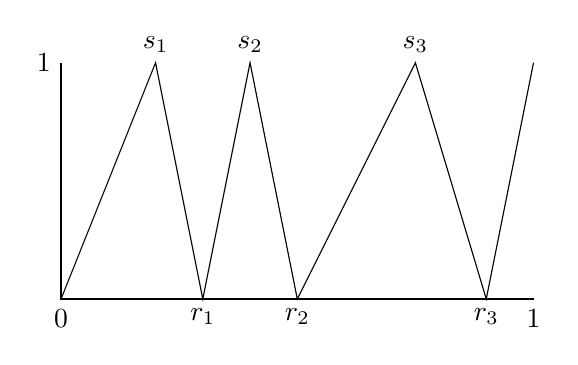
\begin{tikzpicture}[scale = 3, xscale = 2]
		% axis
			\draw[thick] (0, 1) node[left]{$1$} -- (0, 0) node[below]{$0$} -- (1, 0) node[below]{$1$};
		% the line
		\draw (0, 0)
		-- (0.2 , 1) node[above] {$s_1$}
		-- (0.3 , 0) node[below] {$r_1$}
		-- (0.4 , 1) node[above] {$s_2$}
		-- (0.5 , 0) node[below] {$r_2$}
		-- (0.75, 1) node[above] {$s_3$}
		-- (0.9 , 0) node[below] {$r_3$}
		-- (1.0 , 1);
	\end{tikzpicture}
	\caption{Parametrization of sawtooth functions by its vertices and spikes.}
	\label{parametrization of sawtooth functions}
\end{figure}

To describe the closure of~$A$, we will use the following interpolation result.

\begin{proposition}[Interpolation by Sawtooth Functions]
	\label{interpolation via sawtooth functions}
	Let~$n ≥ 1$ be a number of data points, let~$0 < x_1 < \dotsb < x_n < 1$ and let~$y_1, \dotsc, y_n ∈ [0, 1]$.
	There exists a sawtooth function~$f \colon [0, 1] \to [0, 1]$ with~$f x_i = y_i$ for every~$i = 1, \dotsc, n$.
\end{proposition}

\begin{proof}
	Suppose we are given some~$0 < x < 1$ and some~$0 < y < 1$.
	Given~$δ > 0$, there exists a unique line going through the points~$(x - δ, 1)$ and~$(x, y)$.
	This unique line intersects the horizontal line~$ℝ × \{ 1 \}$ at precisely one point, which is of the form~$(x + δ', 0)$ for some~$δ' > 0$, as depicted in \cref{graphical justification for slope formula}.
	We have
	\[
		\frac{y}{δ'} = \frac{1 - y}{δ} \,,
	\]
	and therefore
	\[
		δ' = \frac{y}{1 - y} \, δ \,.
	\]
	\begin{figure}
		\centering
		\begin{tikzpicture}[scale = 3.5, xscale = 1.5];
			% axes
			\draw[thick] (-0.1, 0) node[left] {$0$} -- (1.1, 0);
			\draw[thick] (-0.1, 1) node[left] {$1$} -- (1.1, 1);
			% points
			\draw[fill] (0.2, 1)   ellipse (0.015 and 0.0225) node[above] {$\rightarrow$};
			\draw[fill] (0.5, 0.4) ellipse (0.015 and 0.0225);
			\draw[fill] (0.7, 0)   ellipse (0.015 and 0.0225) node[below] {$\leftarrow$};
			% lines
			\draw (0.5, 0) --node[left] {$y$} (0.5, 0.4) --node[right] {$1 - y$}  (0.5, 1) node[above] {$x$};
			\draw (0.7, 0) -- (0.2, 1);
			% non-visible lines for placement of deltas
			\draw (0.2, 1) --node[above] {$δ$}  (0.5, 1);
			\draw (0.5, 0) --node[below] {$δ'$} (0.7, 0);
		\end{tikzpicture}
		\caption{We have~$y / δ = (1 - y) / δ'$, and as~$δ \to 0$ we also have~$δ' \to 0$.}
		\label{graphical justification for slope formula}
	\end{figure}
	So for~$δ \to 0$ we have also~$δ' \to 0$.

	Let now~$ε > 0$ such that the intervals~$(x_i - ε, x_i + ε)$ are contained in~$[0, 1]$ and pairwise disjoint.
	We define the values~$s_i$ and~$r_i$ as follows:
	\begin{casedistinction}

		\item
			If~$y_i = 0$ then~$s_i ≔ (x_i - ε/2, 1)$ and~$r_i ≔ (x_i, 0) = (x_i, y_i)$.

		\item
			If~$y_i = 1$ then~$s_i ≔ (x_i, 1) = (x_i, y_i)$ and~$r_i ≔ (x_i  + ε/2, 0)$.

		\item
			If~$0 < y_i < 1$, then let~$δ > 0$ be sufficiently small so that both~$δ < ε$ and also~$δ' < ε$ for~$δ' ≔ y / (y - 1) ⋅ δ$.
			We then set~$s_i ≔ (x_i - δ, 1)$ and~$r_i ≔ (x_i + δ', 0)$.

	\end{casedistinction}
	The sawtooth function~$f$ corresponding to the numbers
	\[
		0 < s_1 < r_1 < \dotsb < s_n < r_n < 1
	\]
	satisfies~$f x_i = y_i$ for every~$i = 1, \dotsc, n$.
	See \cref{interpolationg sawtooth function} for an example.
	\begin{figure}
		\[
			\begin{array}{crcr}
				{}
				&
				\centerbox{
				\begin{tikzpicture}[scale = 2.5, xscale = 2]
					% gray areas
					%\draw[fill, gray!30] (0.1, 1) rectangle (0.3, 0);
					%\draw[fill, gray!30] (0.4, 1) rectangle (0.6, 0);
					%\draw[fill, gray!30] (0.7, 1) rectangle (0.9, 0);
					% axes
					\draw[thick] (0, 1) -- (0, 0) -- (1, 0);
					% the points to be interpolated
					\draw[fill] (0.2, 0)   ellipse (0.015 and 0.03);
					\draw[fill] (0.5, 0.5) ellipse (0.015 and 0.03);
					\draw[fill] (0.8, 1)   ellipse (0.015 and 0.03);
					% the intervals with ε = 0.1
					%\draw[(-)] (0.1, -0.2) -- (0.3, -0.2);
					%\draw[(-)] (0.4, -0.2) -- (0.6, -0.2);
					%\draw[(-)] (0.7, -0.2) -- (0.9, -0.2);
				\end{tikzpicture}
				}
				&
				\leadsto
				&
				\centerbox{
				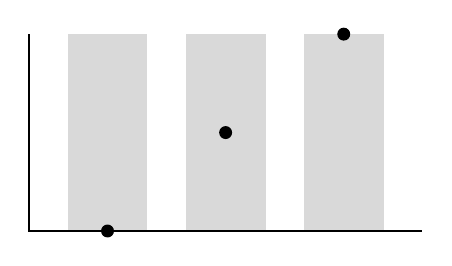
\begin{tikzpicture}[scale = 2.5, xscale = 2]
					% gray areas
					\draw[fill, gray!30] (0.1, 1) rectangle (0.3, 0);
					\draw[fill, gray!30] (0.4, 1) rectangle (0.6, 0);
					\draw[fill, gray!30] (0.7, 1) rectangle (0.9, 0);
					% axes
					\draw[thick] (0, 1) -- (0, 0) -- (1, 0);
					% the points to be interpolated
					\draw[fill] (0.2, 0)   ellipse (0.015 and 0.03);
					\draw[fill] (0.5, 0.5) ellipse (0.015 and 0.03);
					\draw[fill] (0.8, 1)   ellipse (0.015 and 0.03);
					% the intervals with ε = 0.1
					%\draw[(-)] (0.1, -0.2) -- (0.3, -0.2);
					%\draw[(-)] (0.4, -0.2) -- (0.6, -0.2);
					%\draw[(-)] (0.7, -0.2) -- (0.9, -0.2);
				\end{tikzpicture}
				}
				\\[5em]
				\leadsto
				&
				\centerbox{
				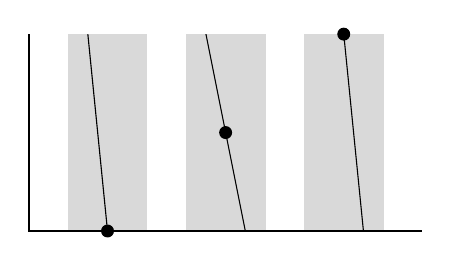
\begin{tikzpicture}[scale = 2.5, xscale = 2]
					% gray areas
					\draw[fill, gray!30] (0.1, 1) rectangle (0.3, 0);
					\draw[fill, gray!30] (0.4, 1) rectangle (0.6, 0);
					\draw[fill, gray!30] (0.7, 1) rectangle (0.9, 0);
					% axes
					\draw[thick] (0, 1) -- (0, 0) -- (1, 0);
					% the points to be interpolated
					\draw[fill] (0.2, 0)   ellipse (0.015 and 0.03);
					\draw[fill] (0.5, 0.5) ellipse (0.015 and 0.03);
					\draw[fill] (0.8, 1)   ellipse (0.015 and 0.03);
					% the intervals with ε = 0.1
					%\draw[(-)] (0.1, -0.2) -- (0.3, -0.2);
					%\draw[(-)] (0.4, -0.2) -- (0.6, -0.2);
					%\draw[(-)] (0.7, -0.2) -- (0.9, -0.2);
					% lines
					\draw (0.15, 1) -- (0.2,  0);
					\draw (0.45, 1) -- (0.55, 0);
					\draw (0.8,  1) -- (0.85, 0);
				\end{tikzpicture}
				}
				&
				\leadsto
				&
				\centerbox{
				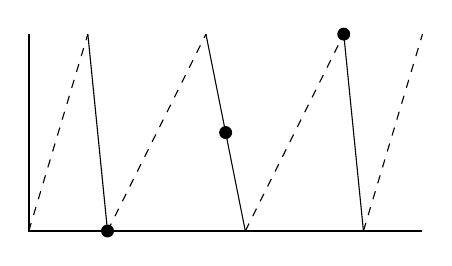
\begin{tikzpicture}[scale = 2.5, xscale = 2]
					% gray areas
					%\draw[fill, gray!30] (0.1, 1) rectangle (0.3, 0);
					%\draw[fill, gray!30] (0.4, 1) rectangle (0.6, 0);
					%\draw[fill, gray!30] (0.7, 1) rectangle (0.9, 0);
					% axes
					\draw[thick] (0, 1) -- (0, 0) -- (1, 0);
					% the points to be interpolated
					\draw[fill] (0.2, 0)   ellipse (0.015 and 0.03);
					\draw[fill] (0.5, 0.5) ellipse (0.015 and 0.03);
					\draw[fill] (0.8, 1)   ellipse (0.015 and 0.03);
					% the intervals with ε = 0.1
					%\draw[(-)] (0.1, -0.2) -- (0.3, -0.2);
					%\draw[(-)] (0.4, -0.2) -- (0.6, -0.2);
					%\draw[(-)] (0.7, -0.2) -- (0.9, -0.2);
					% lines
					\draw (0.15, 1) -- (0.2,  0);
					\draw (0.45, 1) -- (0.55, 0);
					\draw (0.8,  1) -- (0.85, 0);
					\draw[dashed] (0,    0) -- (0.15, 1);
					\draw[dashed] (0.2,  0) -- (0.45, 1);
					\draw[dashed] (0.55, 0) -- (0.8,  1);
					\draw[dashed] (0.85, 0) -- (1,    1);
				\end{tikzpicture}
				}
			\end{array}
		\]
		\caption{A sawtooth function that interpolated between for the three points~$(0.2, 0)$,~$(0.5, 0.5)$ and~$(0.8, 1)$.}
		\label{interpolationg sawtooth function}
	\end{figure}
\end{proof}



\subsubsection{The Closure of~$A$}

Instead of only showing that the zero function lies in the closure in~$A$, we show more generally that~$A$ is dense in~$X$.
To this end, we characterize dense subsets in terms of their intersection with open sets:

\begin{lemma}
	Let~$X$ be a topological space and let~$D$ be a subset of~$X$.
	The set~$D$ is dense in~$X$ if and only if every nonempty open subset of~$X$ intersects~$D$.
\end{lemma}

In other words:
the definition of \enquote{dense} we gave in \cref{definition of dense subsets} is equivalent to the definition given in Section~3.1 the book.

\begin{proof}
	We have the chain of equivalences
	\begin{align*}
		{}&
		\text{$D$ is dense in~$X$} \\
		\iff{}&
		\closure{D} = X \\
		\iff{}&
		\text{the only closed subset of~$X$ that contains~$D$ is~$X$ itself} \\
		\iff{}&
		\text{the only open subset of~$X$ that doesn’t intersect~$D$ is~$∅$} \,,
	\end{align*}
	which proves the assertion.
\end{proof}

Let now~$U$ be any nonempty open subset of~$[0, 1]^{[0, 1]}$.
We need to show that~$A$ intersects~$U$.
For this, we may assume that~$U$ is a basic open set for the product topology, i.e., that there exist distinct points~$x_1, \dotsc, x_n$ in~$[0, 1]$ and open subsets~$U_1, \dotsc, U_n$ of~$[0, 1]$ with
\[
	U
	=
	\{
		f ∈ [0, 1]^{[0, 1]}
		\suchthat
		\text{$f x_i ∈ U_i$ for every~$i$}
	\} \,.
\]
The neighbourhood~$U$ is nonempty, so the sets~$U_i$ must also be nonempty.
For every index~$i$ we choose some point~$y_i$ in~$U_i$.
We know from \cref{interpolation via sawtooth functions} that there exist a sawtooth function~$f$ with~$f x_i = y_i$ for every~$i$, and thus~$f ∈ U$.
This shows that~$U$ intersects~$A$.



\subsubsection{The Zero Function is Not The Limit of a Sequence in~$A$}

\begin{proposition}
	\label{convergece of sequences in products is coordinate-wise}
	Let~$(X_α)_{α ∈ A}$ be a family of topological spaces, let~$(x_n)_n$ be a sequence in~$X ≔ ∏_{α ∈ A} X_α$, and let~$x$ be some point in~$X$.
	Then~$(x_n)_n \to x$ in~$X$ if and only if this holds in each coordinate.
	More explicitly, if~$x_n = (x_n^α)_α$ and~$x = (x^α)_α$, then~$(x_n)_n \to x$ if and only if~$(x_n^α)_α \to x^α$ for every index~$α ∈ A$.
\end{proposition}

\begin{proof}
	For all distinct indices~$α_1, \dotsc, α_r ∈ A$ and all open subsets~$U_i ⊆ X_{α_i}$ we denote the resulting basic open subset of~$X$ by
	\[
		P(U_1, \dotsc, U_r)
		≔
		∏_{α ∈ A}
		\begin{cases*}
			U_i & if~$α = α_i$ for some~$i$, \\
			X_α & otherwise.
		\end{cases*}
	\]
	We have the chain of equivalences
	\begingroup
	\allowdisplaybreaks
	\begin{align*}
		{}&
		(x_n)_n \to x
		\\
		\iff{}&
		\left\{
		\begin{tabular}{l}
			for every open subset~$U$ of~$X$ with~$x ∈ U$, \\
			there exists some~$N$ with~$x_n ∈ U$ for every~$n ≥ N$
		\end{tabular}
		\right.
		\\
		\iff{}&
		\left\{
		\begin{tabular}{l}
			for every basic open subset~$U$ of~$X$ with~$x ∈ U$, \\
			there exists some~$N$ with~$x_n ∈ U$ for every~$n ≥ N$
		\end{tabular}
		\right.
		\\
		\iff{}&
		\left\{
		\begin{tabular}{l}
			for all distinct indices~$α_1, \dotsc, α_r ∈ A$ \\
			and open subsets~$U_i ⊆ X_{α_i}$ with~$x ∈ P(U_1, \dotsc, U_r)$, \\
			there exists some~$N$ with~$x_n ∈ P(U_1, \dotsc, U_r)$ for every~$n ≥ N$
		\end{tabular}
		\right.
		\\
		\iff{}&
		\left\{
		\begin{tabular}{l}
			for all distinct indices~$α_1, \dotsc, α_r ∈ A$ \\
			and open subsets~$U_i ⊆ X_{α_i}$ with~$x^{α_i} ∈ U_i$ for every~$i$, \\
			there exists some~$N$ with~$x_n^{α_i} ∈ U_i$ for all~$i$ and~$n ≥ N$
		\end{tabular}
		\right.
		\\
		\iff{}&
		\left\{
		\begin{tabular}{l}
			for all distinct indices~$α_1, \dotsc, α_r ∈ A$ \\
			and open subsets~$U_i ⊆ X_{α_i}$ with~$x^{α_i} ∈ U_i$ for every~$i$, \\
			there exists some~$N_1, \dotsc, N_r$ with~$x_n^{α_i} ∈ U_i$ for all~$i$ and ~$n ≥ N_i$
		\end{tabular}
		\right.
		\\
		\iff{}&
		\left\{
		\begin{tabular}{l}
			for every index~$α ∈ A$ \\
			and every open subset~$U ⊆ X_α$ with~$x^α ∈ U$, \\
			there exists some~$N$ with~$x_n^α ∈ U$ for every~$n ≥ N$
		\end{tabular}
		\right.
		\\
		\iff{}&
		\text{$(x_n^α)_n \to x^α$ for every~$α ∈ A$} \,.
	\end{align*}
	\endgroup
	This shows the claimed equivalence.
\end{proof}

Suppose there exists a sequence of sawtooth functions~$(f_n)_n$ with~$(f_n)_n \to 0$ with respect to the product topology on~$[0, 1]^{[0, 1]}$.
According to the above \lcnamecref{convergece of sequences in products is coordinate-wise} this is equivalent to~$(f_n)_n \to 0$ pointwise.
However, we will see in the following that this cannot happen, since sawtooth functions are rather rigid:
not too many values of~$f_n$ can tend to~$0$ at the same time.

There exists by assumption for every point~$x$ in~$[0, 1]$ some natural number~$N$ such that~$f_n x ≤ 1/2$ for every~$n ≥ N$.
For every natural number~$N$ let
\[
	B_N
	≔
	\{ x ∈ [0, 1] \suchthat \text{$f_n x ≤ 1/2$ for every~$n ≥ N$} \} \,.
\]
These sets~$B_N$ form an increasing filtration of~$[0, 1]$, i.e., we have
\[
	B_0 ⊆ B_1 ⊆ B_2 ⊆ B_3 ⊆ \dotsb
\]
and~$[0, 1] = ⋃_{N = 0}^∞ B_N$.
We can also describe the sets~$B_N$ in terms of the sets
\[
	B'_n ≔ \{ x ∈ [0, 1] \suchthat f_n x ≤ 1/2 \}
\]
as the intersection~$B_N = ⋂_{n ≥ N} B'_n$.

We note that each set~$B'_n$ is Lebesgue-measurable, since the sawtooth function~$f_n$ is continuous.
Let us calculate the Lebesgue-measure of~$B'_n$:

We observe that for every sawtooth function~$f$ with corresponding points
\[
	0 < s_1 < r_1 < s_2 < r_2 < \dotsb < s_n < r_n < 1 \,,
\]
we have for the set~$B' ≔ \{ x ∈ [0, 1] \suchthat f x ≤ 1/2 \}$ the explicit description
\[
	B'
	=
	\biggl[ 0, \frac{s_1}{2} \biggr]
	∪ \biggl[ \frac{s_1 + r_1}{2}, \frac{r_1 + s_2}{2} \biggr]
	∪ \biggl[ \frac{s_2 + r_2}{2}, \frac{r_2 + s_3}{2} \biggr]
	∪ \dotsb
	∪ \biggl[ \frac{s_n + r_n}{2}, \frac{r_n + 1}{2} \biggr] \,.
\]
See \cref{cutting sawtooth function in half} for a visualization.
\begin{figure}
	\centering
	\begin{tikzpicture}[scale = 3, xscale = 4]
		% coordinates
		\coordinate (0)  at (0,    0);
		\coordinate (s1) at (0.2,  0);
		\coordinate (r1) at (0.3,  0);
		\coordinate (s2) at (0.4,  0);
		\coordinate (r2) at (0.5,  0);
		\coordinate (s3) at (0.75, 0);
		\coordinate (r3) at (0.9,  0);
		% coloured areas
		\draw[fill, gray!50] (0, 0) -- (0.1, 0.5) -- (0.1, 0) -- cycle;
		\draw[fill, gray!50] (0.25, 0) -- (0.25, 0.5) -- (r1) -- (0.35, 0.5) -- (0.35, 0) -- cycle;
		\draw[fill, gray!50] (0.45, 0) -- (0.45, 0.5) -- (r2) -- (0.625, 0.5) -- (0.625, 0) -- cycle;
		\draw[fill, gray!50] (0.825, 0) -- (0.825, 0.5) -- (r3) -- (0.95, 0.5) -- (0.95, 0) -- cycle;
		% the nodes and dashed lines
		\draw[dashed, thick] (0, 1.05) -- ++(0, -1.1) node[below] {$0$};
		\draw[dashed, thick] ($(s1) + (0, 1.05)$) -- ++(0, -1.1) node[below] {$s_1$};
		\draw[dashed, thick] ($(r1) + (0, 1.05)$) -- ++(0, -1.1) node[below] {$r_1$};
		\draw[dashed, thick] ($(s2) + (0, 1.05)$) -- ++(0, -1.1) node[below] {$s_2$};
		\draw[dashed, thick] ($(r2) + (0, 1.05)$) -- ++(0, -1.1) node[below] {$r_2$};
		\draw[dashed, thick] ($(s3) + (0, 1.05)$) -- ++(0, -1.1) node[below] {$s_3$};
		\draw[dashed, thick] ($(r3) + (0, 1.05)$) -- ++(0, -1.1) node[below] {$r_3$};
		\draw[dashed, thick] (1, 1.05) -- ++(0, -1.1) node[below] {$1$};
		% vertical dashed lines
		\draw[dashed, gray!50] (0.1 ,  1.05) -- (0.1,   0);
		\draw[dashed, gray!50] (0.25,  1.05) -- (0.25,  0);
		\draw[dashed, gray!50] (0.35,  1.05) -- (0.35,  0);
		\draw[dashed, gray!50] (0.45,  1.05) -- (0.45,  0);
		\draw[dashed, gray!50] (0.45,  1.05) -- (0.45,  0);
		\draw[dashed, gray!50] (0.625, 1.05) -- (0.625, 0);
		\draw[dashed, gray!50] (0.825, 1.05) -- (0.825, 0);
		\draw[dashed, gray!50] (0.95 , 1.05) -- (0.95 , 0);
		% horizontal dashed lines
		%\draw[dashed, gray!50] (-0.02, 0.5) -- (1.02, 0.5);
		% axis
		\draw[thick] (0, 1) node[left]{$1$} -- (0, 0) -- (1, 0);
		% the line
		\draw (0) -- ($(s1) + (0, 1)$) -- (r1) -- ($(s2) + (0, 1)$) -- (r2) -- ($(s3) + (0, 1)$) -- (r3) -- (1.0 , 1);
	\end{tikzpicture}
	\caption{An explicit description of those points~$x$ with~$f x ≤ 1 / 2$.
	The graph is a triangle in each interval~$[0, s_1], [s_1, r_1], \dotsc, [r_3, 1]$, so we take half of each interval.}
	\label{cutting sawtooth function in half}
\end{figure}
It follows that
\[
	λ B'
	=
	\frac{s_1}{2} + \frac{s_2 - s_1}{2} + \frac{s_3 - s_2}{2} + \dotsb + \frac{1 - s_n}{2}
	=
	\frac{1}{2} \,.
\]
We find in particular that
\[
	λ B'_n = \frac{1}{2}
\]
for every~$n$.

We find now that on the one hand
\[
	λ B_N ≤ λ B'_N ≤ \frac{1}{2}
\]
for every~$N$.
But since the sets~$B_N$ form an increasing filtration of~$[0, 1]$, we also find on the other hand
\[
	λ B_N \to λ [0, 1] = 1 \,.
\]
This is a contradiction!

\subsection{Exercise~3.5}



\subsubsection{a)}

The book forgot to define what a subnet is.
As discussed in \cite[§Subnets]{nlab_subnets}, there are multiple non-equivalent definitions.
We will use the strongest of these definitions, as this ensures that our solutions will also work with the other, weaker definitions.

\begin{definition}
	Let~$P$ and~$Q$ be two preordered sets.
	A map~$f$ from~$P$ to~$Q$ is \defemph{final} if for every element~$y$ of~$Y$ there exists some element~$x$ of~$X$ with~$f x ≥ y$.
\end{definition}

\begin{definition}
	\label{definition of subnet}
	Let~$X$ be a set and let~$(x_α)_{α ∈ D}$ be a set in~$X$.
	Let~$D'$ be another directed set and let~$φ$ be an isotone, final function from~$D$ to~$D'$.
	The net~$(x_{φ β})_{β ∈ D'}$ is a \defemph{subnet} of the net~$(x_α)_{α ∈ D}$.
\end{definition}

We can now solve the given exercise.

A subsequence of a sequence~$(x_n)_{n ∈ ℕ}$ is, by definition, a sequence~$(x_{k_i})_{i ∈ ℕ}$ where~$k \colon ℕ \to ℕ$ is strictly isotone.
This entails that~$k_i ≥ i$ for every~$i ∈ ℕ$, whence~$k$ is not only isotone but also final.
The subsequence~$(x_{k_i})_{i ∈ ℕ}$ is therefore also a subnet.

There are different kinds of examples of subnets of sequences that are not subsequences.
\begin{itemize*}

	\item
		Let~$(x_n)_{n ∈ ℕ}$ be any sequence in~$X$.
		We regard~$ℕ × ℕ$ as a poset with the product order:~$(n, m) ≤ (n', m')$ if and only if both~$n ≤ n'$ and~$m ≤ m'$.
		This poset is directed since~$ℕ$ is directed.
		The map
		\[
			φ \colon ℕ × ℕ \to ℕ \,, \quad (n, m) \mapsto n + m
		\]
		is isotone and final.
		The resulting subnet
		\[
			(x_{φ (n, m)})_{(n, m) ∈ ℕ × ℕ} = (x_{n + m})_{(n, m) ∈ ℕ × ℕ}
		\]
		is not a subsequence, since it is not indexed by~$ℕ$ anymore.

	\item
		One might object that the above counterexample \enquote{is cheating} since the considered subnet is not even a sequence anymore.
		We give therefore another example.

		Let~$(x_n)_{n ∈ ℕ}$ be a sequence in~$X$ with no repeating values.
		This entails that its subsequences also have no repeating values.
		Let~$φ \colon ℕ \to ℕ$ be the map with values
		\[
			0 \,, \enspace 0 \,, \enspace
			1 \,, \enspace 1 \,, \enspace
			2 \,, \enspace 2 \,, \enspace
			3 \,, \enspace 3 \,, \enspace
			4 \,, \enspace 4 \,, \enspace
			5 \,, \enspace 5 \,, \enspace
			\dotsc
		\]
		The sequence~$(x_{φ n})_{n ∈ ℕ}$ repeats every value twice, and can therefore not be a subsequence of the original sequence~$(x_n)_{n ∈ ℕ}$.

	\item
		One might object that the above counterexample is still somewhat artificial:
		it only occurs because in the definition of a subsequence we require~$k \colon ℕ \to ℕ$ to be strictly isotone, whereas in the definition of a subnet we allow~$φ \colon D' \to D$ to be non-strictly isotone.
		We could therefore try to find a subnet~$(x_{φ α})_{α ∈ D}$ of a sequence~$(x_n)_n$ with~$D = ℕ$ and~$φ$ is injective.
		But then~$φ$ would already be strictly isotone, and so the subnet would be a subsequence.

\end{itemize*}

If we were to consider a weaker notion of subnets, then other problems could also occur.

\begin{definition}
	Let~$P$ and~$Q$ be two preordered sets.
	A map~$f$ from~$P$ to~$Q$ is \defemph{strongly final} if for every element~$y$ of~$Q$ there exists an element~$x$ of~$P$ with~$f x' ≥ y$ for every~$x' ≥ x$.
\end{definition}

\begin{itemize*}[resume*]

	\item
		Some authors require the map~$φ$ in the definition of a subnet to only be strongly final.%
		\footnote{
			Every isotone, final map is also strongly final.
			This alternative definition of a subnet is therefore weaker/more general than \cref{definition of subnet}.
		}
		In this case, we can consider the map~$φ \colon ℕ \to ℕ$ given by the values
		\[
			1 \,, \enspace 0 \,, \enspace
			3 \,, \enspace 2 \,, \enspace
			5 \,, \enspace 4 \,, \enspace
			7 \,, \enspace 6 \,, \enspace
			9 \,, \enspace 8 \,, \enspace
			11 \,, \enspace 10 \,, \enspace
			\dotsc
		\]
		In other words, the map~$φ$ swaps the two elements~$2n$ and~$2n + 1$ for every~$n ∈ ℕ$.
		This map is strongly final and injective.
		But if~$(x_n)_n$ is once again a sequence without repeating values, then once again the subnet~$(x_{φ n})_{n ∈ ℕ}$ of~$(x_n)_n$ will not be a subsequence.

\end{itemize*}



\subsubsection{b)}

We have for every element~$(A, a)$ of~$\mathcal{D}$ the inclusion~$A ⊆ A$ and therefore the inequality~$(A, a) ≤ (A, a)$.

Let~$(A, a)$,~$(B, b)$ and~$(C, c)$ be elements of~$\mathcal{D}$ with~$(A, a) ≤ (B, b) ≤ (C, c)$.
Then~$C ⊆ B ⊆ A$, therefore~$C ⊆ A$, and thus~$(A, a) ≤ (C, c)$.

Let~$(A, a)$ and~$(B, b)$ be two arbitrary elements of~$\mathcal{D}$.
The sets~$A$ and~$B$ belong to the filter~$\filter{F}$, whence their intersection~$A ∩ B$ again belongs to~$\filter{F}$.
This intersection must be nonempty, since the filter~$\filter{F}$ is proper (and therefore does not contain the empty set).
There hence exists some element~$x$ in~$A ∩ B$.
The pair~$(A ∩ B, x)$ is an element of~$\mathcal{D}$ with both~$(A, a) ≤ (A ∩ B, x)$ and~$(B, b) ≤ (A ∩ B, x)$.



\subsubsection{c)}

Every set~$A$ belonging to~$\filter{F}$ is nonempty, whence there exists some element~$a$ with~$(A, a) ∈ \mathcal{D}$.
We have for every subset~$C$ of~$X$ the chain of equivalences
\begin{align}
	{}&
	C ∈ \event_{π_{\filter{F}}}
	\notag \\
	\iff{}&
	\left\{
	\begin{tabular}{l}
		there exists some~$(A, a) ∈ \mathcal{D}$ \\
		with~$π_{\filter{F}} (B, b) ∈ C$ for every~$(B, b) ∈ \mathcal{D}$ with~$(B, b) ≥ (A, a)$
	\end{tabular}
	\right.
	\notag \\
	\iff{}&
	\left\{
	\begin{tabular}{l}
		there exists some~$A ∈ \filter{F}$ \\
		with~$b ∈ C$ for every~$B ∈ \filter{F}$ with~$B ⊆ A$ and every~$b ∈ B$
	\end{tabular}
	\right.
	\notag \\
	\iff{}&
	\left\{
	\begin{tabular}{l}
		there exists some~$A ∈ \filter{F}$ \\
		with~$B ⊆ C$ for every~$B ∈ \filter{F}$ with~$B ⊆ A$
	\end{tabular}
	\right.
	\notag \\
	\iff{}&
	\label{translate to intersections}
	\text{there exists some~$A ∈ \filter{F}$ with~$B' ∩ A ⊆ C$ for every~$B' ∈ \filter{F}$} \\
	\iff{}&
	\label{use upward closed}
	C ∈ \filter{F} \,.
\end{align}
For the equivalence~\eqref{translate to intersections} we use that~$\filter{F}$ is closed under intersections, and for the equivalence~\eqref{use upward closed} we use that~$\filter{F}$ is upward closed.



\subsubsection{d)}

Let~$\top{T}$ be the topology on~$X$.
We have for every point~$x$ in~$X$ the chain of equivalences
\[
	π_{\filter{F}} \to x
	\iff
	\top{T}_x ⊆ \event_{π_{\filter{F}}}
	\iff
	\top{T}_x ⊆ \filter{F}
	\iff
	\filter{F} \to x \,.
\]

\subsection{Exercise~3.6}
\label{exercise 3.6}



\subsubsection{The Map~$I$ is Not Continuous}

If~$I$ were continuous then the preimage~$U ≔ I^{-1} [0, 1)$ would be a nonempty open subset of~$Y$.
There would hence exist a basic open set~$V$ of~$[0, 1]^{[0, 1]}$ such that~$Y ∩ V$ is nonempty and~$Y ∩ V ⊆ U$.
There then exist distinct points~$x_1, \dotsc, x_n$ of~$[0, 1]$ and open subsets~$V_1, \dotsc, V_n$ of~$[0, 1]$ such that
\[
	V
	=
	\{
		f \colon [0, 1] \to [0, 1]
		\suchthat
		f(x_i) ∈ \text{$V_i$ for every~$i$}
	\} \,.
\]
It follows that
\[
	Y ∩ V
	=
	\{
		f ∈ Y
		\suchthat
		f(x_i) ∈ \text{$V_i$ for every~$i$}
	\} \,.
\]
The set~$V$ is nonempty, so each~$V_i$ is nonempty.
We choose for every index~$i$ some point~$y_i$ in~$V_i$ and consider the function
\[
	f
	\colon
	[0, 1] \to [0, 1] \,,
	\quad
	x
	\mapsto
	\begin{cases*}
		y_i & if~$x = x_i$ for some~$i$, \\
		1   & otherwise.
	\end{cases*}
\]
This function is contained in~$Y$ and has~$I f = 1$, since it is constant with value~$1$ almost everywhere.
But~$f$ is also contained in~$Y ∩ V$ and thus in~$U$, whence~$I f < 1$.
A contradiction!



\subsubsection{The Map~$I$ Preserves Convergence of Sequences}

Let~$(f_n)_n$ be a sequence in~$Y$ with~$(f_n)_n \to f$ for some function~$f$ in~$Y$.
According to \cref{convergece of sequences in products is coordinate-wise} (page~\pageref{convergece of sequences in products is coordinate-wise}) this means that the sequence~$(f_n)_n$ converges pointwise to~$f$.

The functions~$f_n$ are dominated by the function with constant value~$1$, which is again integrable.
It follows from the dominated convergence theorem that~$I f_n = ∫_0^1 f_n \to ∫_0^1 f = I f$ as~$n \to ∞$.

\subsection{Exercise~3.7}

The set~$X$ belongs to~$\filter{F}$, and we have~$f X = Y$.
Therefore,~$Y$ belongs to the proposed filterbase, which entails that it is nonempty.

Let~$B$ and~$B'$ be two sets belonging to the proposed filterbase.
This means that there exist sets~$A$ and~$A'$ belonging to~$\filter{F}$ with~$f A ⊆ B$ and~$f A' ⊆ B'$.
The intersection~$A ∩ A'$ again belongs to~$\filter{F}$, and we have
\[
	f (A ∩ A')
	⊆
	f A ∩ f A'
	⊆
	B ∩ B' \,.
\]
This tells us that the intersection~$B ∩ B'$ is again contained in the proposed filterbase, which shows that it is downward directed.

\subsection{Exercise~3.8}
\label{exercise 3.8}

Let~$B$ be a subset of~$Y$ not belonging to~$f_* \filter{F}$.
This means that the preimage~$f^{-1} B$ does not belong to~$\filter{F}$.
There hence exists by Proposition~3.1 a set~$A$ belonging to~$\filter{F}$ with~$A ∩ f^{-1} B = ∅$.
This means that no point of~$A$ is mapped into~$B$ by the map~$f$, whence~$f A ∩ B = ∅$.
But the set~$f A$ is contained in~$f_* \filter{F}$.

According to Proposition~3.1, we have shown that the filter~$f_* \filter{F}$ is again an ultrafilter.

\subsection{Exercise~3.9}



\subsubsection{Hausdorff implies KC}

We have seen that in Corollary~2.18.1 that in a Hausdorff space, compact subspaces are closed.



\subsubsection{KC does not imply Hausdorff}

We consider an uncountable set~$X$ with the cocountable topology, i.e., the closed subsets of~$X$ are the countable subsets and the entire space.
We have seen in Exercise~3.2 that~$X$ is not a Hausdorff space (since it is uncountable).

But we claim that every infinite set~$Y$ together with the cocountable topology is a KC space.

We observe that for every subspace~$Z$ of~$Y$, the topology on~$Z$ is again the cocountable topology.
Consequently, if~$Z$ is infinite, then it is not compact:
there then exists an infinite sequence~$z_0, z_1, z_2, \dotsc$ of pairwise distinct points in~$Z$, and the closed subsets~$C_n ≔ \{ z_k \suchthat k ≥ n \}$ of~$Z$ satisfy the Finite Intersection Property even though the overall intersection~$⋂_{n ≥ 0} C_n$ is empty.

The compact subspaces of~$Y$ are therefore precisely the finite subspaces, all of which are closed in~$Y$.



\subsubsection{KC implies US}

\begin{lemma}
	\label{compact spaces from convergent sequences}
	Let~$X$ be a topological space and let~$(x_n)_n$ be a convergent sequence in~$X$ with limit~$x$.
	The subspace~$\{ x_n \suchthat n ≥ 0 \} ∪ \{ x \}$ of~$X$ is compact.
\end{lemma}

\begin{proof}
	We denote the proposed set by~$K$.
	Let~$\cover{U}$ be a cover of~$K$ by open subsets of~$X$.
	There exists some set~$U_∞$ belonging to~$\cover{U}$ with~$x ∈ U_∞$, and there exists some~$N$ with~$x_n ∈ U_∞$ for every~$n ≥ N$.
	There exists for every~$n = 0, \dotsc, N - 1$ some set~$U_n$ belonging to~$\cover{U}$ with~$x_n ∈ U_n$.
	We have thus found a finite subcover of~$\cover{U}$, namely~$\{ U_0, \dotsc, U_{N - 1}, U_∞ \}$.
\end{proof}

Let~$X$ be a KC space.

For every point~$x$ in~$X$, the singleton space~$\{ x \}$ is compact, and therefore closed in~$X$.
This tells us that~$x$ is the unique limit of the constant sequence~$x, x, x, \dotsc$

Let now~$(x_n)_n$ be a sequence in~$X$ that converges to two points~$x$ and~$y$.
For every~$N$, the truncated sequence~$(x_n)_{n ≥ N}$ again converges to~$x$.
Therefore, the set~$K_n ≔ \{ x_n \suchthat n ≥ N \} ∪ \{ x \}$ is compact by the above \lcnamecref{compact spaces from convergent sequences}, and thus closed because~$X$ is a KC space.
It follows from Theorem~3.3 that~$y$ is contained in each~$K_n$.
It follows that either~$x = y$ or there exist infinitely many indices~$n$ with~$x_n = y$.
In the second case, the constant sequence~$y, y, y, \dotsc$ is a subsequence of~$(x_n)_n$ and therefore again converges to~$x$.
But we have already seen that~$y$ is the unique limit of~$y, y, y, \dotsc$
So~$x = y$ even in the second case.



\subsubsection{US does not imply KC}

Let~$ω_1$ be the first uncountable ordinal.
We will make use of the following properties of~$ω_1$:
\begin{enumerate*}

	\item
		$ω_1$ is a linear poset.%
		\footnote{
			By \enquote{linear} we mean that any two elements are comparable.
		}

	\item
		$ω_1$ is, in fact, well-ordered:
		every nonempty subset of~$ω_1$ admits a least element.%
		\footnote{
			Well-ordered posets are necessarily linear, since for every two elements~$x$ and~$y$ the set~$\{ x, y \}$ admits a least element.
			If this least element is~$x$, then~$x ≤ y$, and otherwise~$y ≤ x$.
		}

	\item
		$ω_1$ is uncountable as a set.

	\item
		For every element~$α$ of~$ω_1$, the set~$\{ β ∈ ω_1 \suchthat β ≤ α \}$ is only countable.

\end{enumerate*}

\begin{definition}
	For every poset~$P$ let~$P^+$ be the extension of~$P$ to a poset with underlying set~$P ⨿ \{ -∞, ∞ \}$ and additional inequalities~$-∞ < x$ and~$x < ∞$ for every~$x ∈ P$.
\end{definition}

We note that for every linear poset~$L$, the extended poset~$L^+$ is again linear.
If~$W$ is a well-ordered poset, then the poset~$W^+$ will again be well-ordered.

\begin{definition}
	Let~$L$ be a linear poset.
	For every two elements~$x$ and~$y$ of~$L^+$, the open interval~$(x, y)$ is given by
	\[
		(x, y) ≔ \{ z ∈ L \suchthat x < z < y \} \,.
	\]
\end{definition}

Finite intersections of open intervals are again open intervals, whence the collection of open intervals is a basis for a topology.

\begin{definition}
	Let~$L$ be a linear poset.
	The \defemph{order topology} on~$L$ is the topology with basis given by all open intervals in~$L$.
\end{definition}

\begin{proposition}
	\label{order topology is hausdorff}
	Let~$L$ be a linear set endowed with the order topology.
	Then~$L$ is a Hausdorff space.
\end{proposition}

\begin{proof}
	Let~$x$ and~$y$ be two distinct elements of~$L$ with~$x < y$.
	We distinguish between two cases.

	Suppose first that there exists an element~$z$ of~$L$ with~$x < z < y$.
	Then the half-open intervals~$(-∞, z)$ and~$(z, ∞)$ are disjoint open neighbourhoods of~$x$ and~$y$ respectively.

	Suppose now that such an element~$z$ does not exist.
	Then the half-open intervals~$(-∞, y)$ and~$(x, ∞)$ are disjoint open neighbourhoods of~$x$ and~$y$ respectively.
\end{proof}

The ordinal~$ω_1$ has the useful property that it cannot be exhausted by any single sequence:

\begin{lemma}
	\label{cannot exhaust omega by a sequence}
	There exists for every sequence~$(x_n)_n$ in~$ω_1$ an element~$y$ of~$ω_1$ with~$y > x_n$ for every index~$n$.
\end{lemma}

\begin{proof}
	Let~$(x_n)_n$ be an arbitrary sequence in~$ω_1$.
	For every index~$n$, the half-open interval~$(-∞, x_n]$ is countable.
	Consequently, the union~$⋃_{n ≥ 0} {} (-∞, x_n]$ is again countable.
	But~$ω_1$ is uncountable, so there exists some element~$y$ of~$ω_1$ not contained in this union.
	This element satisfies~$y > x_n$ for every index~$n$.
\end{proof}

Let us now consider the poset~$ω_1 + 1$ that arises from~$ω_1$ by adding a new element~$Ω$ with~$Ω > x$ for every~$x ∈ ω_1$.
We note that~$ω_1 + 1$ is again well-ordered.

\begin{corollary}
	\label{Omega is not a limit from below}
	A sequence in~$ω_1 + 1$ converges to the point~$Ω$ (with respect to the order topology) if and only if it is eventually constant with value~$Ω$.
\end{corollary}

\begin{proof}
	If the sequence~$(x_n)_n$ is eventually constant with value~$Ω$, then~$(x_n)_n$ converges to~$Ω$.

	Let conversely~$(x_n)_n$ be any sequence in~$ω_1 + 1$ that is not eventually constant with value~$Ω$.
	The sequence~$(x_n)_n$ then admits a subsequence~$(x_{k_i})_i$ that never takes on the value~$Ω$ at all.
	This means that the subsequence~$(x_{k_i})_i$ is entirely contained in~$ω_1$.
	It follows from \cref{cannot exhaust omega by a sequence} that there exists some element~$y$ of~$ω_1$ with~$y > x_{k_i}$ for every index~$i$.
	The open interval~$(y, ∞)$ is an open neighbourhood of~$Ω$ that doesn’t contain any term of the subsequence~$(x_{k_i})_i$, whence this subsequence doesn’t converge to~$Ω$.
	Consequently, the original sequence~$(x_n)_n$ doesn’t converge to~$Ω$.
\end{proof}

We observe that by adding the point~$Ω$ to~$ω_1$, the resulting space becomes compact.

\begin{lemma}
	\label{compactness of bounded ordinals}
	Let~$W$ be a well-ordered poset admitting a greatest element~$Ω$.
	Then~$W$ is compact in the order topology.
\end{lemma}

\begin{proof}
	Let~$\cover{U}$ be an open cover of~$W$ and let
	\[
		S
		≔
		\left\{
			x ∈ W^+
			\suchthat*
			\begin{tabular}{l}
				the open interval~$(x, ∞)$ can be covered \\
				by finitely many sets belonging to~$\cover{U}$
			\end{tabular}
		\right\} \,.
	\]
	The set~$S$ is nonempty since it contains~$∞$, because~$(∞, ∞) = ∅$.
	The poset~$W^+$ is again well-ordered, because~$W$ is well-ordered, whence the set~$S$ admits a least element~$s$.

	The greatest element~$Ω$ of~$W$ is also contained in~$S$, since~$(Ω, ∞) = ∅$.
	We have therefore~$s < Ω < ∞$, so either~$s = -∞$ or~$s ∈ W$.
	If~$s = -∞$ then we find that~$(s, ∞) = (-∞, ∞) = W$ admits a finite subcover.
	
	Suppose now that~$s ∈ W$.
	There exist finitely many sets~$U_1, \dotsc, U_n$ belonging to~$\cover{U}$ that cover~$(s, ∞)$.
	But because~$s ∈ W$ there also exists an open set~$U_0$ belonging to~$\cover{U}$ with~$s ∈ U_0$.
	This open set~$U_0$ contains an open interval~$(x, y)$ around~$s$, where~$x, y ∈ W^+$ with~$x < y$.
	We find that~$(x, ∞) = (x, y) ∪ (s, ∞)$ is covered by the finitely many sets~$U_0, \dotsc, U_n$, whence~$x ∈ S$.
	But~$x < s$ since~$s ∈ (x, y)$, and~$s$ is the minimal element of~$S$.
	A contradiction!
\end{proof}

We see that the space~$ω_1 + 1$ together with the order topology is a compact Hausdorff space, but that the additional point~$Ω$ of~$ω_1 + 1$ cannot be reached by sequences in~$ω_1$.
We can therefore destroy the Hausdorff property without changing the sequential properties of the space~$ω_1 + 1$.
For this, we will use the following general construction (\cref{duplicating a point}).

\begin{lemma}
	\label{factorization of quotient map}
	Consider the following diagram of topological spaces and continuous maps:
	\[
		\begin{tikzcd}[column sep = small]
			X
			\arrow{rr}[above]{f}
			\arrow{dr}[below left]{h}
			&
			{}
			&
			Y
			\arrow{dl}[below right]{g}
			\\
			{}
			&
			Z
			&
			{}
		\end{tikzcd}
	\]
	Suppose the map~$f$ is a surjective quotient map.
	Then the map~$g$ is a surjective quotient map if and only if the composite~$h = g f$ is a surjective quotient map.
\end{lemma}

\begin{proof}
	We have~$g Y = g f X = h X$ by the surjectivity of~$f$, whence~$g$ is surjective if and only if~$h$ is surjective.
	We have also the chain of equivalences
	\begin{align*}
		{}&
		\text{$g$ is a quotient map}
		\\
		\iff{}&
		\left\{
		\begin{tabular}{l}
			for every topological space~$W$ and every map~$k \colon Z \to W$, \\
			the map~$k$ is continuous if and only if the map~$k g$ is continuous
		\end{tabular}
		\right.
		\\
		\iff{}&
		\left\{
		\begin{tabular}{l}
			for every topological space~$W$ and every map~$k \colon Z \to W$, \\
			the map~$k$ is continuous if and only if the map~$k g f$ is continuous
		\end{tabular}
		\right.
		\\
		\iff{}&
		\left\{
		\begin{tabular}{l}
			for every topological space~$W$ and every map~$k \colon Z \to W$, \\
			the map~$k$ is continuous if and only if the map~$k h$ is continuous
		\end{tabular}
		\right.
		\\
		\iff{}&
		\text{$h$ is a quotient map} \,.
	\end{align*}
	This proves the assertion.
\end{proof}

\begin{proposition}[Duplicating a point]
	\label{duplicating a point}
	Let~$X$ be a topological space and let~$x_0$ be a point in~$X$ such that the singleton set~$\{ x_0 \}$ is closed.
	Let
	\[
		Y ≔ ( X ∖ x_0 ) ⨿ \{ x_1, x_2 \}
	\]
	and let~$\top{T}$ be the collection of subsets of~$Y$ consisting of the following sets:
	\begin{itemize*}

		\item
			Those open subsets of~$X$ not containing~$x$.

		\item
			For every open subset~$U$ of~$X$ containing~$x$ the three sets
			\[
				(U ∖ x_0) ∪ \{ x_1 \} \,,
				\quad
				(U ∖ x_0) ∪ \{ x_2 \} \,,
				\quad
				(U ∖ x_0) ∪ \{ x_1, x_2 \} \,.
			\]

	\end{itemize*}
	Then the following hold:
	\begin{enumerate}

		\item
			The collection~$\top{T}$ is a topology on~$Y$.

		\item
			The subspace~$Y ∖ x_1$ is homeomorphic to~$X$ by identifying~$x_2$ with~$x$.
			Similarly, the subspace~$Y ∖ x_2$ is homeomorphic to~$X$ by identifying~$x_1$ with~$x$.

		\item
			The map from~$Y$ to~$X$ that identifies both~$x_1$ and~$x_2$ with the original point~$x$ is a quotient map.

	\end{enumerate}
\end{proposition}

\begin{proof}
	We denote the points of the coproduct~$X ⨿ X$ by~$(x, i)$ with~$x ∈ X$ and~$i ∈ \{ 1, 2 \}$, indicating in which summand the point lies.

	\begin{enumerate}

		\item
			Let~$∼$ be the equivalence relation on~$X ⨿ X$ that identifies for every point~$x$ of~$X$ with~$x ≠ x_0$ the two points~$(x, 1)$ and~$(x, 2)$, and let~$Y' ≔ (X ⨿ X) / {∼}$.

			The open subsets of~$Y'$ correspond to open saturated subsets of~$X ⨿ X$.
			These open saturated sets are the following, see \cref{four kinds of open saturated sets}.
			\begin{itemize*}

				\item
					For every open subset~$U$ of~$X$ not containing~$x_0$ the set~$U ⨿ U$.

				\item
					For every open subset~$U$ of~$X$ containing~$x_0$ the three sets
					\[
						(U ∖ x_0) ⨿ U \,, \quad U ⨿ (U ∖ x_0) \,, \quad U ⨿ U \,.
					\]
					(We use here that~$\{ x_0 \}$ is closed, to conclude that~$U ∖ x_0$ is again open.)

			\end{itemize*}
			\begin{figure}
				\centering
				\begin{tikzpicture}[scale = 1.2]
					% lines
					\draw (-1, 0) -- (1, 0);
					\draw (-1, 1) -- (1, 1);
					% points
					\draw[fill] (0, 0) circle (0.04);
					\draw[fill] (0, 1) circle (0.04);
					% open sets
					\draw[(-), thick] (-0.8, 0) -- (-0.2, 0);
					\draw[(-), thick] ( 0.8, 0) -- ( 0.2, 0);
					\draw[(-), thick] (-0.8, 1) -- (-0.2, 1);
					\draw[(-), thick] ( 0.8, 1) -- ( 0.2, 1);
				\end{tikzpicture}
				\qquad
				\begin{tikzpicture}[scale = 1.2]
					% lines
					\draw (-1, 0) -- (1, 0);
					\draw (-1, 1) -- (1, 1);
					% points
					\draw[fill] (0, 0) circle (0.04);
					\draw[fill] (0, 1) circle (0.04);
					% open sets
					\draw[(-), thick] (-0.6, 0) -- (0.6, 0);
					\draw[(-), thick] (-0.6, 1) -- (-0.04, 1);
					\draw[(-), thick] (0.04, 1) -- (0.6, 1);
				\end{tikzpicture}
				\qquad
				\begin{tikzpicture}[scale = 1.2]
					% lines
					\draw (-1, 0) -- (1, 0);
					\draw (-1, 1) -- (1, 1);
					% points
					\draw[fill] (0, 0) circle (0.04);
					\draw[fill] (0, 1) circle (0.04);
					% open sets
					\draw[(-), thick] (-0.6, 0) -- (-0.04, 0);
					\draw[(-), thick] (0.04, 0) -- (0.6, 0);
					\draw[(-), thick] (-0.6, 1) -- (0.6, 1);
				\end{tikzpicture}
				\qquad
				\begin{tikzpicture}[scale = 1.2]
					% lines
					\draw (-1, 0) -- (1, 0);
					\draw (-1, 1) -- (1, 1);
					% points
					\draw[fill] (0, 0) circle (0.04);
					\draw[fill] (0, 1) circle (0.04);
					% open sets
					\draw[(-), thick] (-0.6, 0) -- (0.6, 0);
					\draw[(-), thick] (-0.6, 1) -- (0.6, 1);
				\end{tikzpicture}
				\caption{The four kinds of open saturated subsets of~$X ⨿ X$.}
				\label{four kinds of open saturated sets}
			\end{figure}
			The open subsets of~$Y'$ are therefore the following:
			\begin{itemize*}

				\item
					For every open subset~$U$ of~$X$ not containing~$x_0$ the set
					\[
						\{ [x, 1] \suchthat x ∈ U \}
						=
						\{ [x, 2] \suchthat x ∈ U \} \,.
					\]

				\item
					For every open subset of~$X$ containing~$x_0$ the three sets
					\begin{gather*}
						\{ \class{x, 1} \suchthat x ∈ U, x ≠ x_0 \} ∪ \{ \class{x_0, 2} \}
						=
						\{ \class{x, 2} \suchthat x ∈ U \} \,, \\
						\{ \class{x, 2} \suchthat x ∈ U, x ≠ x_0 \} ∪ \{ \class{x_0, 1} \}
						=
						\{ \class{x, 1} \suchthat x ∈ U \} \,, \\
						\{ \class{x, 1} \suchthat x ∈ U, x ≠ x_0 \} ∪ \{ \class{x_0, 1}, \class{x_0, 2} \} \,.
					\end{gather*}

			\end{itemize*}

			We have a bijection between~$Y$ and~$Y'$:
			for every point~$x$ of~$X$ with~$x ≠ x_0$, the point~$x$ in~$Y$ corresponds to the point~$\class{x, 0} = \class{x, 1}$ in~$Y'$;
			the two points~$x_1$ and~$x_2$ in~$Y$ correspond to the points~$\class{x_0, 1}$ and~$\class{x_0, 2}$ in~$Y'$ respectively.
			Under this bijection, the open subsets of~$Y'$ correspond precisely to the sets belonging to~$\top{T}$.
			Therefore,~$\top{T}$ is a topology on~$Y$.

		\item
			It follows from the explicit description of~$\top{T}$ and the explicit description of the subspace topology that~$Y ∖ x_1$ has the following open subsets:
			\begin{itemize*}

				\item
					Every open subset of~$X$ that doesn’t contain the point~$x$ is also an open subset of~$Y ∖ x_1$.

				\item
					For every open subset~$U$ of~$X$ that contains the point~$x$, the sets
					\begin{gather*}
						( (U ∖ x_0) ∪ \{ x_1 \} ) ∖ x_1 = U ∖ x_0 \,,
						\\
						( (U ∖ x_0) ∪ \{ x_2 \} ) ∖ x_1 = (U ∖ x_0) ∪ \{ x_2 \} \,,
						\\
						( (U ∖ x_0) ∪ \{ x_1, x_2 \} ) ∖ x_1 = (U ∖ x_0) ∪ \{ x_2 \}
					\end{gather*}
					are open in~$Y ∖ x_1$.

			\end{itemize*}
			The open subsets of~$Y ∖ x_1$ are hence the open subsets of~$X$, but with~$x$ replaced by~$x_2$.
			Consequently, the map from~$X$ to~$Y ∖ x_1$ that replaces~$x$ with~$x_2$ is a homeomorphism.

			For~$Y ∖ x_2$ the argumentation is the same.

		\item
			Let~$∇$ be the codiagonal map from~$X ⨿ X$ to~$X$, given by~$∇ (x, i) = x$ for every point~$x$ in~$X$ and every~$i = 1, 2$.
			The map~$∇$ is continuous, and it factors through a continuous map~$p$ from~$Y'$ to~$X$.

			The map~$∇$ is in fact a quotient map, since for every subset~$U$ of~$X$, the set~$U$ is open in~$X$ if and only if its preimage~$∇^{-1} U = U ⨿ U$ is open in~$X ⨿ X$.
			It follows from \cref{factorization of quotient map} that the map~$p$ is again a quotient map.
			Under the homeomorphism between~$Y'$ and~$Y$, the surjective quotient map~$p$ corresponds to the proposed map that identifies~$x_1$ and~$x_2$ with~$x$.
		\qedhere

	\end{enumerate}
\end{proof}

\begin{example}
	Duplicating the point~$0$ of the real line~$ℝ$ results in the line with two origins.
\end{example}

We consider now the space~$X ≔ ω_1 + 1$ with its special point~$Ω$.
We use \cref{duplicating a point} to replace the point~$Ω$ by two points~$Ω_1$ and~$Ω_2$, resulting in a topological space~$Y$ whose underlying set is given by~$ω_1 ⨿ \{ Ω_1, Ω_2 \}$.

We observe that for every point~$y$ in~$Y$, the singleton set~$\{ y \}$ is closed:
If~$y ∈ ω_1$, then~$\{ y \}$ is closed in~$X$ because~$X$ is a Hausdorff space;
consequently,~$X ∖ y$ is open in~$X$, whence~$((X ∖ y) ∖ Ω) ∪ \{ Ω_1, Ω_2 \}$ is open in~$Y$;
but this set is just~$Y ∖ y$.
If~$y = Ω_1$, then~$Y ∖ y = (X ∖ Ω) ∪ \{ Ω_2 \}$ is open in~$Y$ because~$X$ is open in~$X$.
For~$y = Ω_2$ we can argue in the same way.

The subspace~$Y ∖ Ω_1$ of~$Y$ is homeomorphic to~$X$, which is compact by \cref{compactness of bounded ordinals}.
But~$Y ∖ Ω_1$ is not closed in~$Y$ because~$\{ Ω_1 \}$ is not open in~$Y$, since~$\{ Ω \}$ is not open in~$X$.
Therefore,~$Y$ is not a KC space.

Limits of sequences in~$Y$ are still unique, making~$Y$ a US space.

To see this, let~$(x_n)_n$ be a sequence in~$Y$ with limits~$x$ and~$y$.
Let~$p$ be the surjective quotient map from~$Y$ to~$X$ that identifies the two points~$Ω_1$ and~$Ω_2$ back into the single point~$Ω$.
The sequence~$(p x_n)_n$ in~$X$ converges to~$p x$ and to~$p y$ by the continuity of~$p$.
Limits in~$X$ are unique, because~$X$ is a Hausdorff space, so~$p x = p y$.
This tells us that either~$x, y ∈ ω_1$ with~$x = y$ or~$x, y ∈ \{ Ω_1, Ω_2 \}$.

In the second case we have~$p x, p y = Ω$.
We have seen above that the sequence~$(p x_n)_n$ is thus eventually constant with value~$Ω$.
Consequently, the original sequence~$(x_n)_n$ is eventually contained in~$p^{-1} Ω = \{ Ω_1, Ω_2 \}$.
This entails that the sequence~$(x_n)_n$ admits a constant subsequence~$(x_{k_i})_i$.
This subsequence also converges to both~$x$ and~$y$, but we have already seen that limits of constant sequences in~$Y$ are unique.
Therefore,~$x = y$.

